
\documentclass[12pt,a4paper]{article}

% -------------------------
% Lingua, codifica, font
% -------------------------
\usepackage[T1]{fontenc}
\usepackage[utf8]{inputenc}
\usepackage[italian]{babel}
\usepackage{lmodern}
\usepackage{microtype}

% -------------------------
% Impaginazione
% -------------------------
\usepackage[a4paper,top=2.7cm,bottom=2.7cm,left=3cm,right=3cm]{geometry}
\usepackage{setspace}
\setstretch{1.05}
\setlength{\parindent}{0pt}
\setlength{\parskip}{0.35em}

% -------------------------
% Matematica, tabelle, figure
% -------------------------
\usepackage{amsmath,amssymb,bm}
\usepackage{graphicx}
\usepackage{float}
\usepackage{booktabs}
\usepackage{array}
\usepackage{caption}
\usepackage{subcaption}
\usepackage{longtable}
\usepackage{multirow}
\usepackage{siunitx}
\sisetup{output-decimal-marker={,}}

% -------------------------
% Codice MATLAB / Simulink
% -------------------------
\usepackage{xcolor}
\usepackage{listings}
\lstdefinestyle{matlabstyle}{
    language=Matlab,
    basicstyle=\ttfamily\small,
    numbers=left,
    numberstyle=\tiny,
    stepnumber=1,
    numbersep=8pt,
    frame=single,
    breaklines=true,
    columns=fullflexible,
    showstringspaces=false,
    keywordstyle=\bfseries,
    commentstyle=\itshape,
    captionpos=b
}

% -------------------------
% Link e riferimenti
% -------------------------
\usepackage[hidelinks]{hyperref}
\usepackage[nameinlink,noabbrev]{cleveref}

% -------------------------
% Stile didascalie e nomi
% -------------------------
\captionsetup{font=small,labelfont=bf,labelsep=colon}
\addto\captionsitalian{\renewcommand{\figurename}{Figura}}
\addto\captionsitalian{\renewcommand{\tablename}{Tabella}}

% -------------------------
% Comandi utili
% -------------------------
\newcommand{\vect}[1]{\bm{#1}}
\newcommand{\mat}[1]{\bm{#1}}
\newcommand{\transp}{^{\top}}
\newcommand{\placeholder}[1]{\textit{#1}}

\begin{document}

% =========================================================
% FRONTESPIZIO
% =========================================================
\begin{titlepage}
    \centering
    \vspace*{2.5cm}

    \begin{figure}[H]
    \centering
    \includegraphics[width=0.9\textwidth]{figures/Logo_UNIPI.jpg}
    %\caption{Andamento delle componenti dello stato nello scenario di validazione.}
    \label{fig:Logo}
    \end{figure}


    {\Large \textbf{Identificazione e Stima}}\\[1.2cm]
    {\Large \textbf{Stima dello stato di un elicottero 2 DoF mediante EKF ed UKF}}\\[3.0cm]
   % {\large Sottotitolo o traccia del progetto}\\[2.0cm]

    \begin{center}
    \large
    Francesco Bonciani 578902 \\
    Edoardo Di Scalzo 603117  \\
    Luigi Realacci 616067
    \end{center}

    \vfill
    {\large Anno Accademico 2025/2026}
\end{titlepage}

\tableofcontents
\newpage


\section{Introduzione}
L'obiettivo del presente progetto è la progettazione e la validazione di
algoritmi di stima dello stato applicati ad un sistema dinamico
non lineare rappresentato da un elicottero a due gradi di libertà (2DOF).
Il sistema considerato descrive i moti di beccheggio (($\alpha$))
e imbardata (($\beta$)) di una piattaforma sperimentale azionata da due motori
elettrici, il cui comportamento è caratterizzato da accoppiamenti dinamici,
attriti viscosi e non linearità trigonometriche.
L'attività è stata sviluppata in ambiente MATLAB/Simulink
ed ha previsto la realizzazione di un modello fisico del sistema,
la simulazione della sensoristica di bordo e l'implementazione di differenti algoritmi di stima 
basati sul filtro di Kalman. In particolare sono stati sviluppati un Filtro di Kalman Esteso (EKF),
un Filtro di Kalman Unscented (UKF) ed uno smoother di Rauch-Tung-Striebel (RTS),
con l'obiettivo di confrontarne prestazioni,
robustezza numerica e accuratezza nella ricostruzione dello stato.
L'architettura di stima utilizza misure provenienti da un accelerometro e da un magnetometro,
modellati a partire dalle specifiche di un sensore reale VectorNav VN-100.
Particolare attenzione è stata dedicata alla gestione di misure asincrone,
alla presenza di outlier e alla validazione statistica delle innovazioni mediante
test di bianchezza e distanza di Mahalanobis.
I risultati ottenuti consentono di valutare l'efficacia dei diversi approcci di sensor
fusion in presenza di dinamiche non lineari e rumori di processo e misura, evidenziandone vantaggi,
limiti e possibili sviluppi futuri.


\section{Implementazione e validazione del modello}
L'elicottero considerato è costituito da una struttura rigida vincolata a ruotare attorno a due assi ortogonali,
consentendo i soli moti di pitch e yaw come mostrato in Figura \ref{fig:Schema_Elicottero}.

\begin{figure}[H]
    \centering
    \includegraphics[width=0.7\textwidth]{figures/modello.jpg}
    \caption{Illustrazione del sistema fisico elicottero 2DOF.}
    \label{fig:Schema_Elicottero}
\end{figure}


L'implementazione del modello è stata realizzata mediante blocchi MATLAB Function
all'interno dell'ambiente Simulink come riportato in Figura \ref{fig:Schema_modello_simulink}.
Il modello include gli effetti gravitazionali,
i contributi dissipativi dovuti agli attriti viscosi e gli accoppiamenti dinamici generati
dall'azione simultanea dei due attuatori.

\begin{figure}[H]
    \centering
    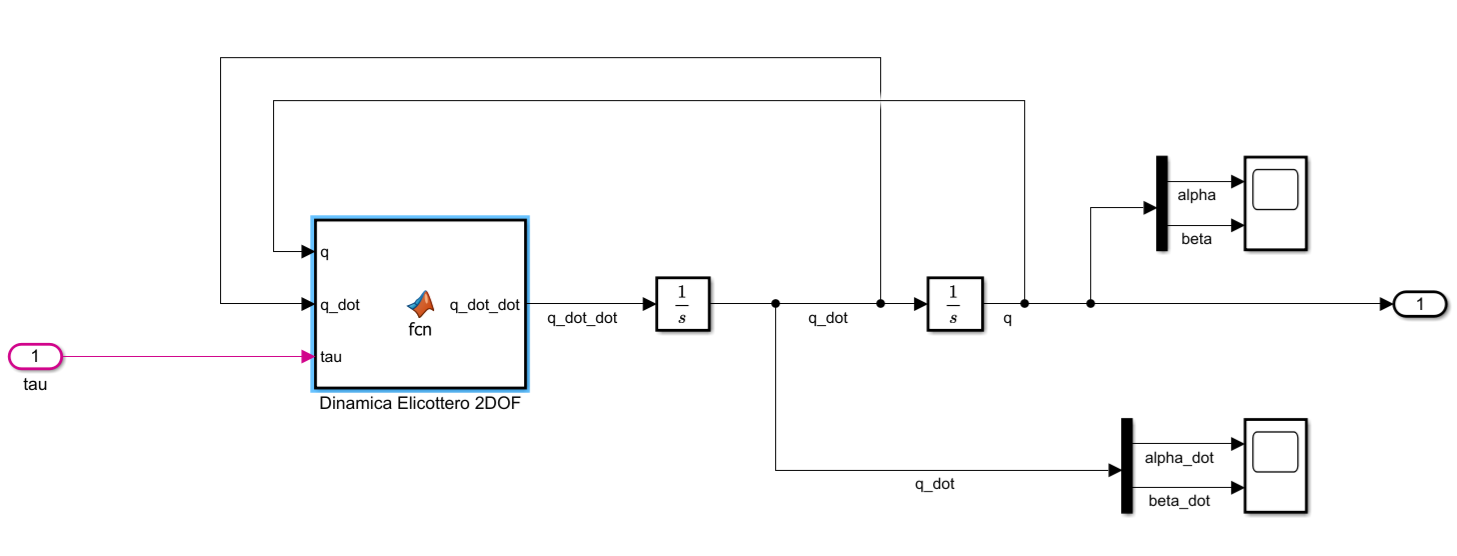
\includegraphics[width=0.8\textwidth]{figures/Schema_simulink_modello.png}
    \caption{Schema Simulink modello del sistema}
    \label{fig:Schema_modello_simulink}
\end{figure}



% Per verificare la correttezza dell'implementazione sono stati eseguiti diversi test di
% simulazione utilizzando ingressi costanti e sinusoidali. In tutti gli scenari considerati
% il comportamento ottenuto è risultato coerente con quello previsto dalle equazioni del moto,
% confermando la correttezza della modellazione e dell'implementazione numerica.



%Le specifiche principali del sistema sono riportate in \cref{tab:specifiche_modello}.

%\begin{table}[H]
%\centering
%\caption{Specifiche del modello.}
%\label{tab:specifiche_modello}
%\begin{tabular}{|>{\centering\arraybackslash}p{4.2cm}|>{\centering\arraybackslash}p{2.2cm}|>{\centering\arraybackslash}p{2.2cm}|>{\centering\arraybackslash}p{3cm}|}
%\hline
%\textbf{Parametro} & \textbf{Simbolo} & \textbf{Valore} & \textbf{Unità di misura} \\
%\hline
%Parametro 1 & $p_1$ & $0.0$ & m \\
%\hline
%Parametro 2 & $p_2$ & $0.0$ & kg \\
%\hline
%Parametro 3 & $p_3$ & $0.0$ & Nms \\
%\hline
%\end{tabular}
%\end{table}

%L'implementazione in ambiente MATLAB/Simulink è composta da \placeholder{numero e tipo di blocchi principali}. In \cref{fig:schema_simulink} è riportato lo schema generale del modello.

%\begin{figure}[H]
   % \centering
   % \includegraphics[width=0.9\textwidth]{figures/placeholder_figure.pdf}
   % \caption{Schema Simulink del modello e dei sensori.}
    %\label{fig:schema_simulink}
%\end{figure}


\subsection{Dinamica}
La dinamica dell'elicottero viene descritta attraverso due coordinate generalizzate, corrispondenti agli angoli di pitch ($\alpha$) e yaw ($\beta$). Il modello deriva dall'applicazione delle equazioni di Eulero-Lagrange ad un sistema meccanico rigido soggetto a forze aerodinamiche e contributi dissipativi.
L'equazione che descrive il moto di pitch è

\begin{equation}
J_{\alpha}\ddot{\alpha} = - c_{\alpha}\dot{\alpha} - mgl\sin(\alpha) + lF_1\cos(\beta) + \varepsilon_p lF_2\sin(\beta)
\end{equation}

dove ($J_{\alpha}$) rappresenta il momento di inerzia rispetto all'asse di pitch, ($m$) è la massa equivalente del sistema, ($g$) l'accelerazione gravitazionale, ($l$) il braccio meccanico dell'elicottero e ($c_{\alpha}$) il coefficiente di attrito viscoso.
L'equazione mostra come il moto di beccheggio sia influenzato da tre contributi principali: la coppia gravitazionale che tende a riportare il sistema verso la posizione di equilibrio, la dissipazione viscosa e la coppia generata dai motori.
L'equazione relativa all'asse di yaw assume invece la forma

\begin{equation}
J_{\beta}(\alpha)\ddot{\beta} = - c_{\beta}\dot{\beta} + lF_2\cos(\alpha) + \varepsilon_y lF_1\sin(\alpha)
\end{equation}

dove il momento di inerzia equivalente attorno all'asse verticale dipende dall'assetto del sistema secondo la relazione

\begin{equation}
J_{\beta}(\alpha) = J_y\sin^2(\alpha) + \left(J_z+ml^2\right)\cos^2(\alpha) + I_b.
\end{equation}

Tale dipendenza introduce una significativa non linearità nel modello e rende particolarmente interessante il confronto tra differenti algoritmi di stima.
Definendo il vettore di stato

\begin{equation}
x = \begin{bmatrix} \alpha & \dot{\alpha} & \beta & \dot{\beta} \end{bmatrix}^{T}
\end{equation}
si ottiene il modello non lineare nello spazio di stato

\begin{equation}
\dot{x}=f(x,u,w)
\end{equation}

con vettore di ingresso 

\begin{equation}
u = [F_1 \quad F_2]^T
\end{equation}

Dove $F_1$ rappresenta la forza del rotore principale ed $F_2$ la forza
del rotore di coda.

La funzione MATLAB visibile in Figura \ref{fig:Schema_modello_simulink} implementa
le equazioni del modello analizzate in precedenza sotto forma di dinamica inversa
secondo l'equazione

\begin{equation}
\ddot{x} = M^{-1}(Bu - n)
\end{equation}

Dove $M$ è la matrice di inerzia

\begin{equation}
    M =
    \begin{bmatrix}
        J_{\alpha} & 0  \\
        0 & J_{\beta}(\alpha)
    \end{bmatrix}
\end{equation}

$B$ è il vettore delle forze generalizzate

\begin{equation}
    B =
    \begin{bmatrix}
        l\cos(\beta) & \epsilon_pl\sin(\beta) \\
        \epsilon_yl\sin(\alpha) & l\cos(\alpha)
    \end{bmatrix}
\end{equation}

ed $n$ raccoglie i termini di attrito viscoso e forza di gravità.

\begin{equation}
    n =
    \begin{bmatrix}
        c_{\alpha}\dot{\alpha} + mgl\sin(\alpha)    \\
        c_{\beta}\dot{\beta}
    \end{bmatrix}
\end{equation}

In Tabella \ref{tab:Parametri} sono illustrati i parametri del sistema.

\begin{table}[H]
\centering
\caption{Specifiche del modello.}
\label{tab:Parametri}
% Nota: Assicurati di aver incluso \usepackage{array} e \usepackage{amsmath} nel preambolo
\begin{tabular}{|>{\centering\arraybackslash}m{4.2cm}|>{\centering\arraybackslash}m{2.2cm}|>{\centering\arraybackslash}m{2.2cm}|>{\centering\arraybackslash}m{3cm}|}
\hline
\textbf{Parametro} & \textbf{Simbolo} & \textbf{Valore} & \textbf{Unità di misura} \\
\hline
Massa & $m$ & $0.2$ & $\text{kg}$ \\
\hline
Braccio delle forze dei rotori & $l$ & $0.2$ & $\text{m}$ \\
\hline
Coefficiente attrito viscoso asse beccheggio & $c_{\alpha}$ & $0.01$ & $\frac{\text{N}\cdot\text{m}\cdot\text{s}}{\text{rad}}$ \\
\hline
Coefficiente attrito viscoso asse imbardata & $c_{\beta}$ & $0.01$ & $\frac{\text{N}\cdot\text{m}\cdot\text{s}}{\text{rad}}$ \\
\hline
Coefficiente di accoppiamento del rotore di coda sull'asse del beccheggio & $\epsilon_p$ & $0.1$ & adim. \\
\hline
Coefficiente di accoppiamento del rotore principale sull'asse di imbardata & $\epsilon_y$ & $0.1$ & adim. \\
\hline
Accelerazione di gravità & $g$ & $9.81$ & $\frac{\text{m}}{\text{s}^2}$ \\
\hline
Momento di inerza rispetto all'asse beccheggio & $J_{\alpha}$ & $0.012$ & $\text{kg}\cdot\text{m}^2$ \\
\hline
Componente di inerzia trasversale & $J_y$ & $0.00023$ & $\text{kg}\cdot\text{m}^2$ \\
\hline
Componente di Inerzia verticale & $J_z$ & $0.00364$ & $\text{kg}\cdot\text{m}^2$ \\
\hline
Componente inerzia della base & $I_b$ & $0.00023$ & $\text{kg}\cdot\text{m}^2$ \\
\hline
\end{tabular}
\end{table}

\subsection{Validazione del modello}
\label{sec:Validazione_modello}
Al fine di verificare la correttezza del modello implementato è stata eseguita una campagna preliminare di simulazioni utilizzando differenti profili di ingresso con componenti costanti per i 2 attuatori.
Tutti i test sono stati effetuati a partire dalle condizioni iniziali
\begin{equation}
    x_0 = [10^\circ \quad 0 \quad 0 \quad 0]^T
\end{equation}

In una prima fase sono stati applicati ingressi nulli
ai due attuatori per osservare la risposta libera del sistema.
Questo ha prodotto gli andamenti del vettore di stato visibili nelle Figure \ref{fig:Input_nulli_angoli} e \ref{fig:Input_nulli_rate}.

\begin{figure}[H]
    \centering
    \includegraphics[width=0.9\textwidth]{figures/validazione_tau_0_0_alpha_beta.png}
    \caption{Andamento angoli di beccheggio ed imbardata con ingressi nulli ai rotori}
    \label{fig:Input_nulli_angoli}
\end{figure}

\begin{figure}[H]
    \centering
    \includegraphics[width=0.9\textwidth]{figures/validazione_tau_0_0_alpha_beta_dot.png}
    \caption{Andamento rate angolari di beccheggio ed imbardata con ingressi nulli ai rotori}
    \label{fig:Input_nulli_rate}
\end{figure}

Da questi andamenti si verifica la correttezza del modello in quanto l'elicottero cade per effetto della gravità
ed oscilla fino a fermarsi intorno al suo equilibrio stabile verticale ($\alpha = 0$).

Successivamente sono stati utilizzati ingressi con componente costante solo su uno dei 2 ingressi per testare i fenomeni di accoppiamento.
Ciò ha prodotto gli andamenti visibili nelle Figure \ref{fig:Input_caso2_angoli}, \ref{fig:Input_caso2_rate}, \ref{fig:Input_caso1_angoli} ed \ref{fig:Input_caso1_rate}.

\begin{figure}[H]
    \centering
    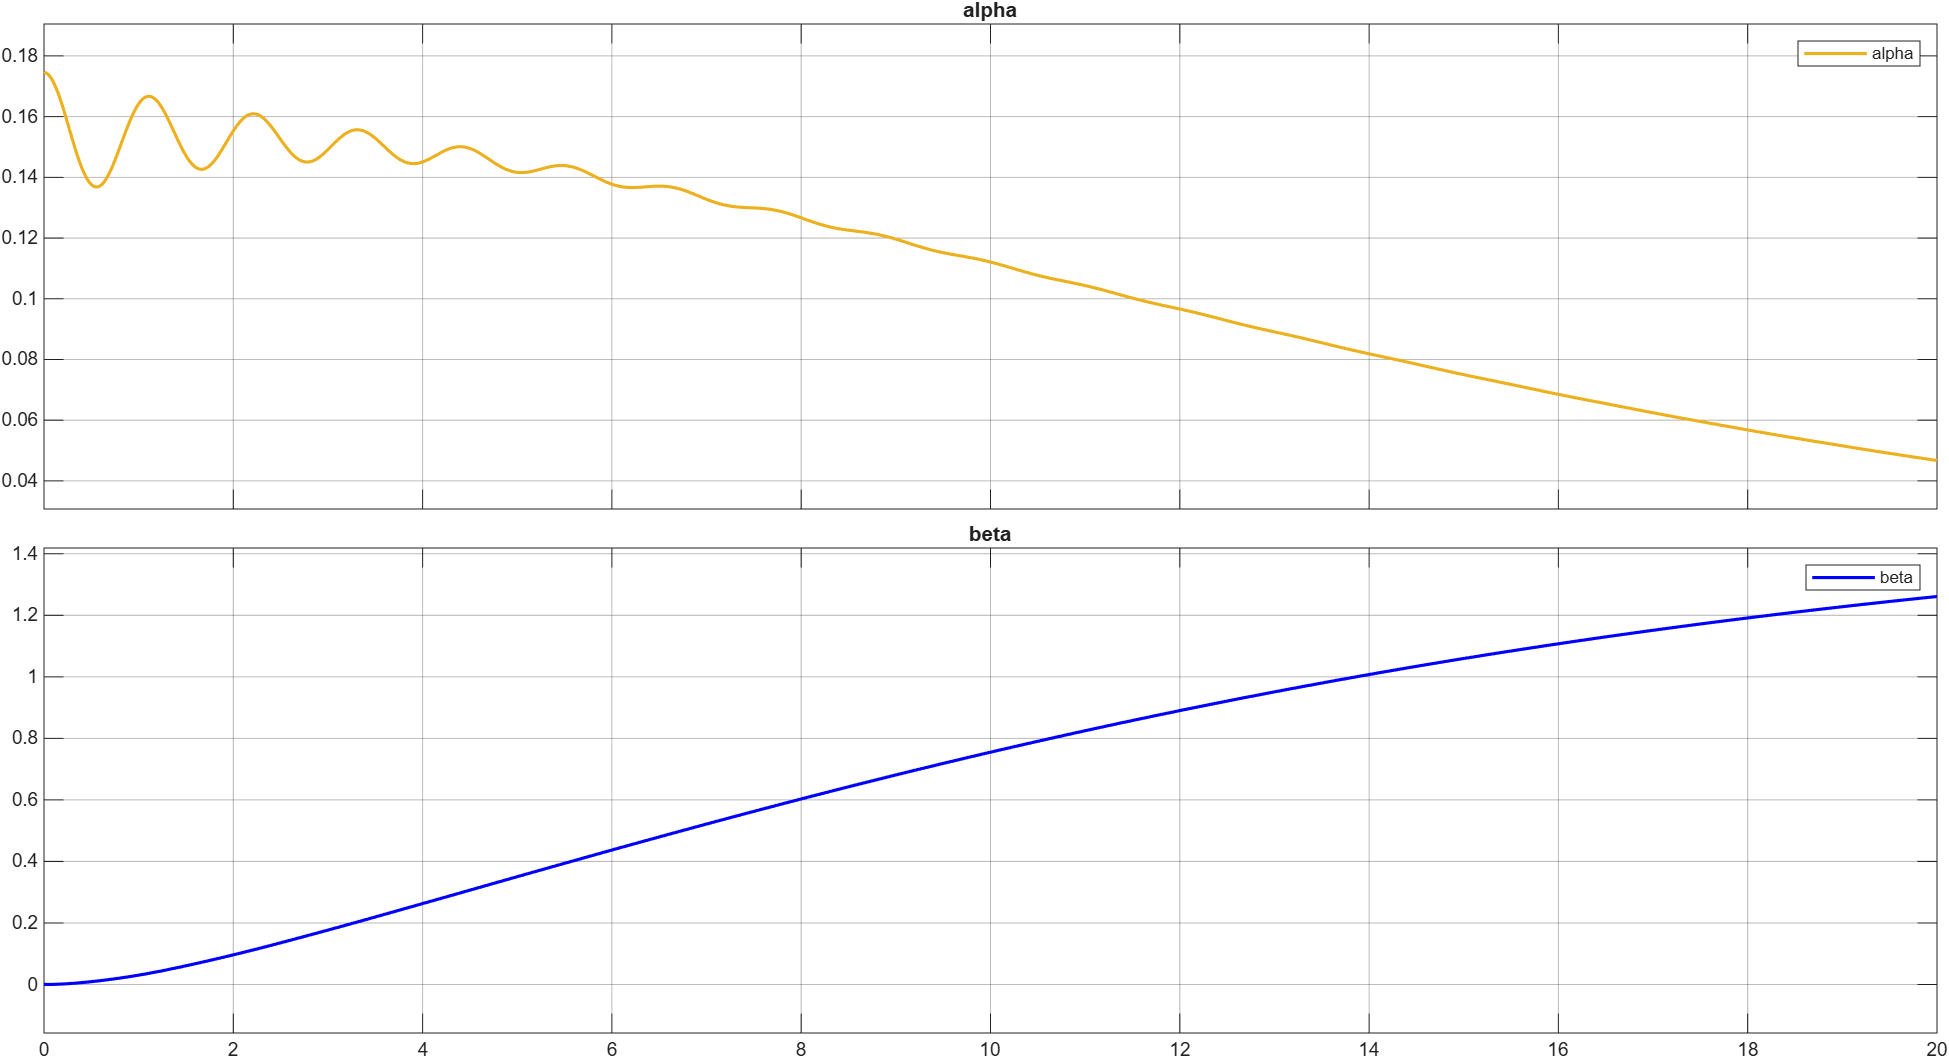
\includegraphics[width=0.9\textwidth]{figures/validazione_tau_1_0_alpha_beta.png}
    \caption{Andamento angoli di beccheggio ed imbardata con ingresso $F_1$ costante}
    \label{fig:Input_caso2_angoli}
\end{figure}

\begin{figure}[H]
    \centering
    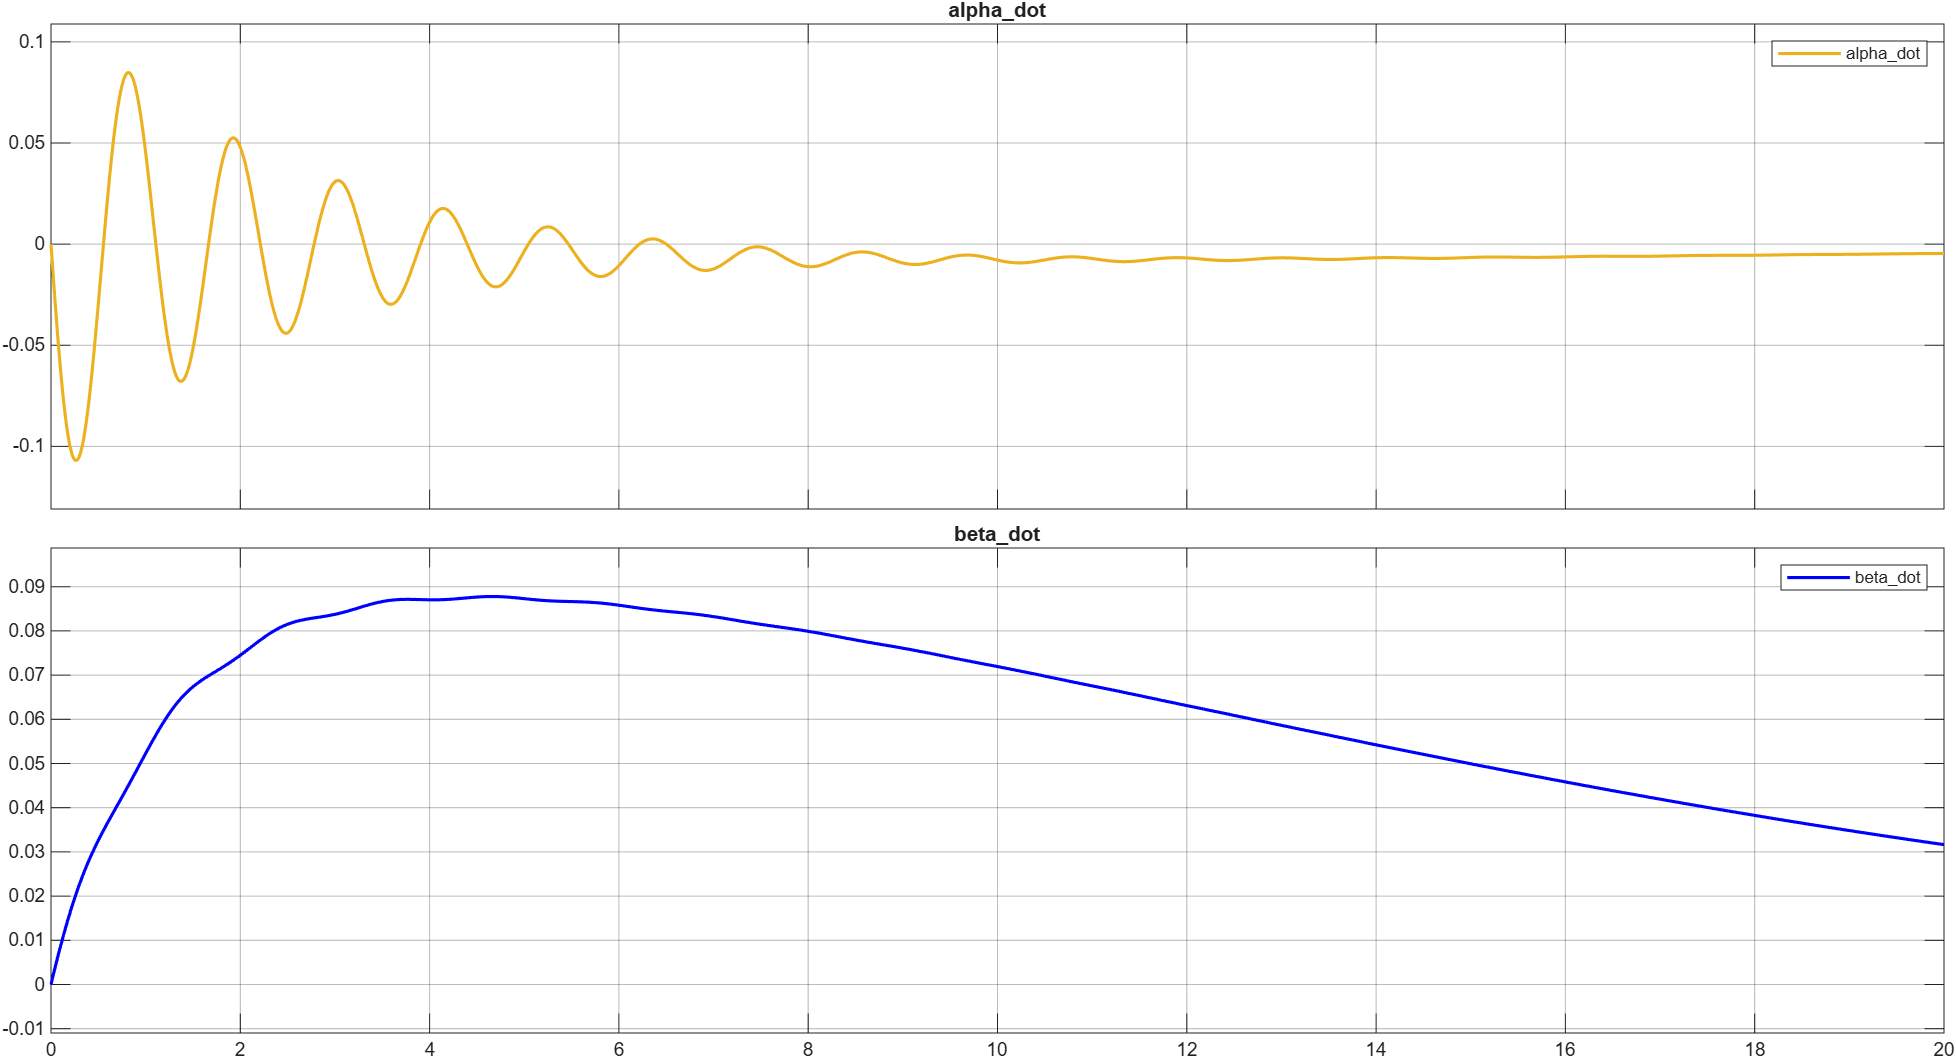
\includegraphics[width=0.9\textwidth]{figures/validazione_tau_1_0_alpha_beta_dot.png}
    \caption{Andamento rate angolari  di beccheggio ed imbardata con ingresso $F_1$ costante}
    \label{fig:Input_caso2_rate}
\end{figure}

Nel primo caso è visibile la risposta all'azionamento del rotore principale ($F_1 = 0.3$ N).
Per quanto riguarda il beccheggio si nota che la forza solleva l'elicottero innescando un transitorio oscillante.
Tali oscillazioni vengono smorzate per effetto dell'attrito viscoso. Contestualmente, si osserva 
un lento abbassamento dell'angolo $\alpha$: man mano che l'elicottero cambia il suo orientamento la spinta del rotore
principale perde di efficacia verticale ($F_1\cos(\beta)$) confermando l'accopiamento geometrico del modello.
Pur non avendo fornito alcun ingresso al rotore di coda, si osserva che l'elicottero inizia spontaneamente a ruotare 
su se stesso. Questo comportamento valida l'accopiamento aerodinamico tra i rotori.



\begin{figure}[H]
    \centering
    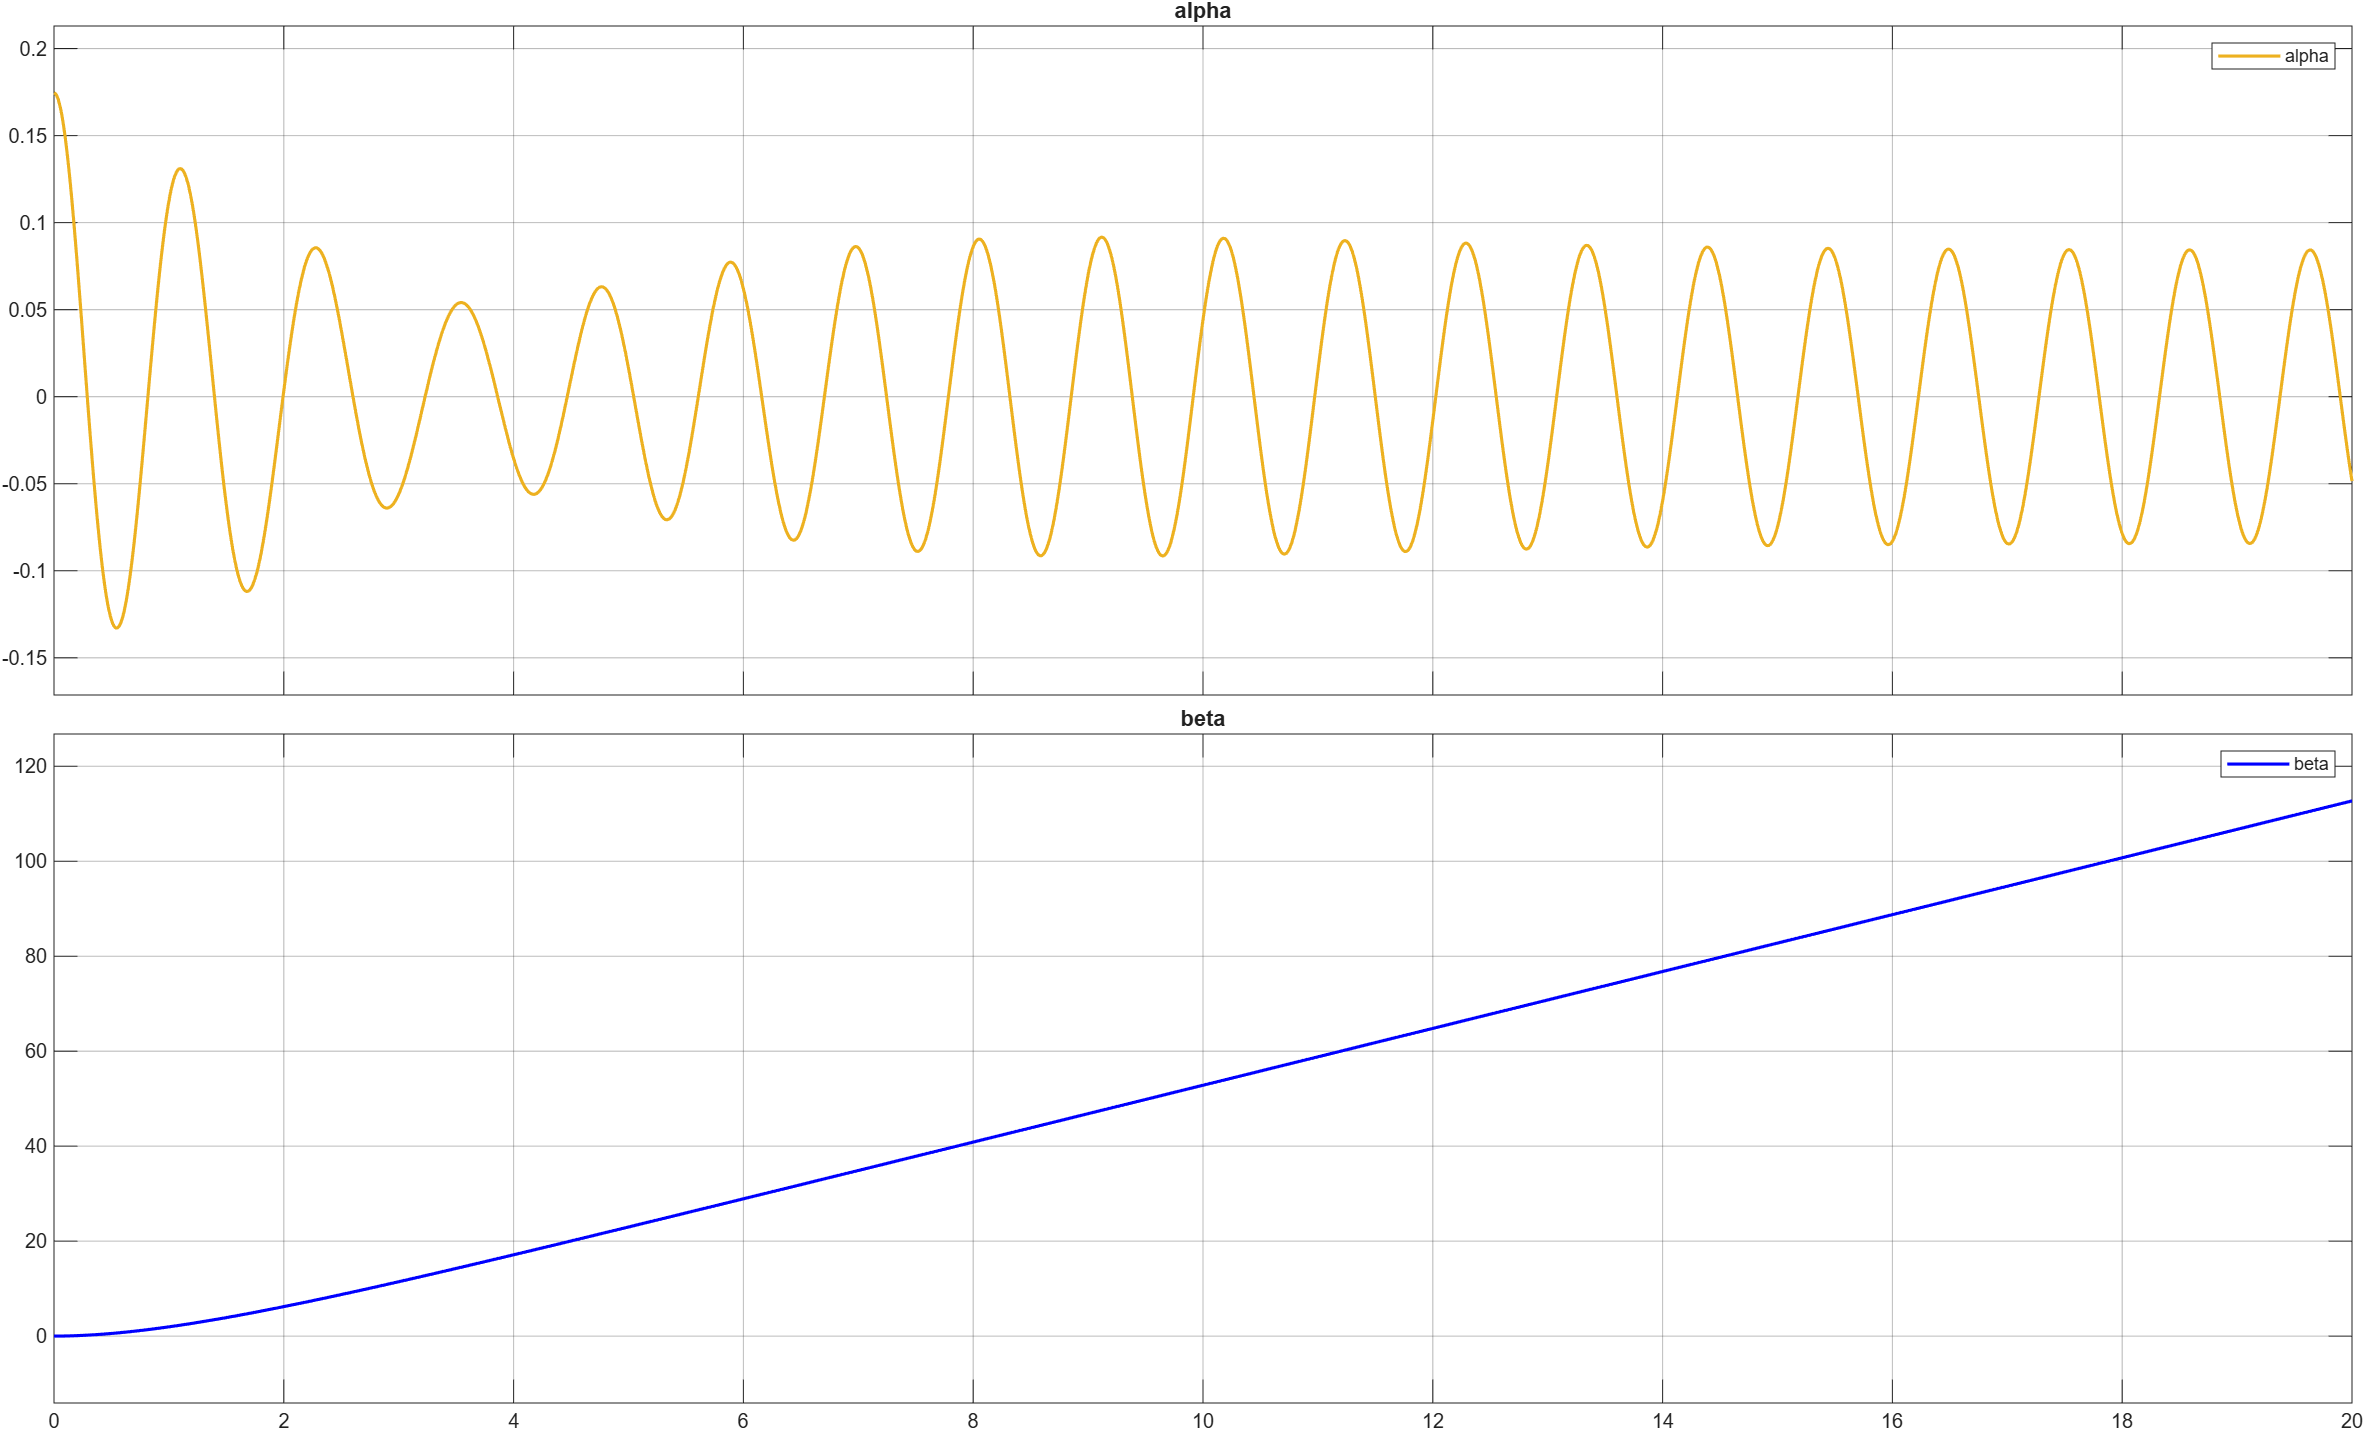
\includegraphics[width=0.9\textwidth]{figures/validazione_tau_0_1_alpha_beta.png}
    \caption{Andamento angoli di beccheggio ed imbardata con ingresso $F_2$ costante}
    \label{fig:Input_caso1_angoli}
\end{figure}

\begin{figure}[H]
    \centering
    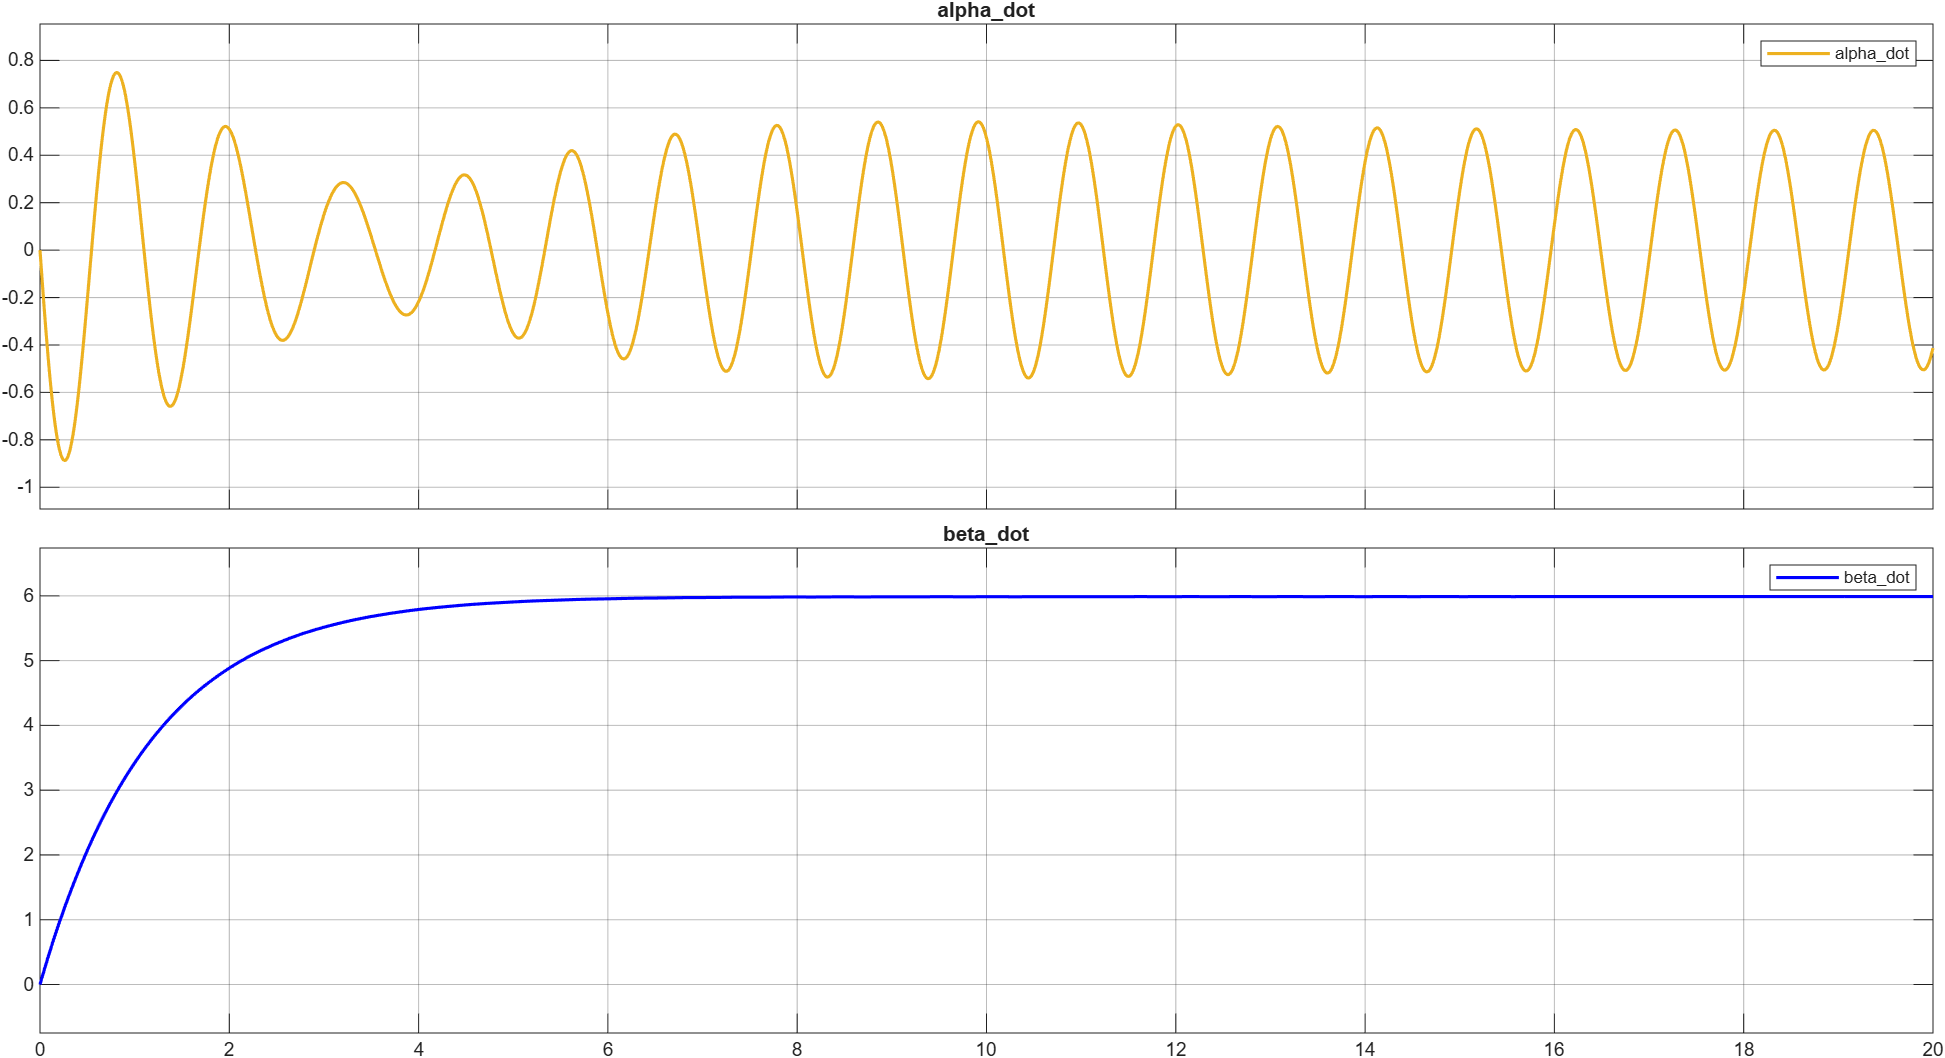
\includegraphics[width=0.9\textwidth]{figures/validazione_tau_0_1_alpha_beta_dot.png}
    \caption{Andamento rate angolari di beccheggio ed imbardata con ingresso $F_2$ costante}
    \label{fig:Input_caso1_rate}
\end{figure}

Nel secondo test l'elicottero viene sollecitato accendendo solamente il rotore di coda ($F_2 = 0.3$ N).
Essendo privo di un richiamo gravitazionale, l'applicazione di una forza costante genera una rotazione continua 
sull'asse dell'imbardata.
L'elicottero accelera fino a quando la coppia impressa dall'elica di coda viene perfettamente
bilanciata dalla resistenza aerodinamica e dall'attrito viscoso.
I grafici della simulazione mostrano infatti una velocità angolare che sale
e si stabilizza in modo pulito a un valore di crociera costante,
confermando la bontà della dinamica del primo ordine implementata per l'orientamento.
Pur essendo il rotore principale spento, l'angolo di pitch entra in un'oscillazione continua.
Ciò valida l'accoppiamento teorico tra gli assi.

\subsection{Sensori}
La stima dello stato viene effettuata sfruttando misure provenienti da un accelerometro e da un magnetometro,
modellati sulla base delle specifiche del sensore inerziale VectorNav VN-100,
visibile in Figura \ref{fig:IMU}.

\begin{figure}[H]
    \centering
    \includegraphics[width=0.7\textwidth]{figures/vectornav_VN100.png}
    \caption{Sensore inerziale VectorNav VN-100}
    \label{fig:IMU}
\end{figure}


L'accelerometro viene utilizzato per ricavare una misura indiretta dell'angolo di pitch attraverso la relazione
\[
y_{acc}=g\sin(\alpha)+v_{acc}
\]
dove (g) rappresenta l'accelerazione gravitazionale e ($v_{acc}$) è un rumore gaussiano a media nulla.
La stima dell'angolo di yaw viene invece ottenuta mediante il magnetometro, il cui modello di osservazione è espresso come
\[
y_{magn}=
[M_0\cos(\beta)\quad
-M_0\sin(\beta)]^T
+
v_{magn}
\]
dove ($M_0 = 46.5$ $\mu\text{T}$) rappresenta il modulo del campo magnetico terrestre locale e ($v_{magn}$) è il rumore di misura associato.
I due sensori operano a frequenze differenti e generano pertanto un problema di fusione dati multi-rate.
L'accelerometro fornisce aggiornamenti a frequenza superiore rispetto al magnetometro; di conseguenza i filtri di stima sono stati progettati in modo da eseguire
la fase di correzione utilizzando esclusivamente le misure effettivamente disponibili all'istante corrente.
In Tabella \ref{tab:Specifiche_sensori} sono riportate le specifiche per ciascun sensore.
Per aumentare il realismo della simulazione sono stati introdotti rumori gaussiani e misure 
spurie generate casualmente(outlier). 
Tali anomalie vengono successivamente identificate e rigettate mediante un test basato sulla
distanza di Mahalanobis. Nelle Figure \ref{fig:Schema_simulink_acc} e \ref{fig:Schema_simulink_magn} sono riportati
gli schemi Simulink implementati per simulare i sensori.

\begin{table}[H]
\centering
\caption{Specifiche dei sensori.}
\label{tab:Specifiche_sensori}
\begin{tabular}{|>{\centering\arraybackslash}m{4.2cm}|>{\centering\arraybackslash}m{3.5cm}|>{\centering\arraybackslash}m{3.5cm}|}
\hline
\textbf{Sensore} & \textbf{Dev. Standard rumore} & \textbf{Frequenza di lavoro} \\
\hline
Accelerometro & 0.0137 $\frac{\text{m}}{\text{s}^2}$ & $230$ Hz \\
\hline
Magnetometro & 0.14 $\mu\text{T}$ & $200$ Hz \\
\hline
\end{tabular}
\end{table}


\begin{figure}[H]
    \centering
    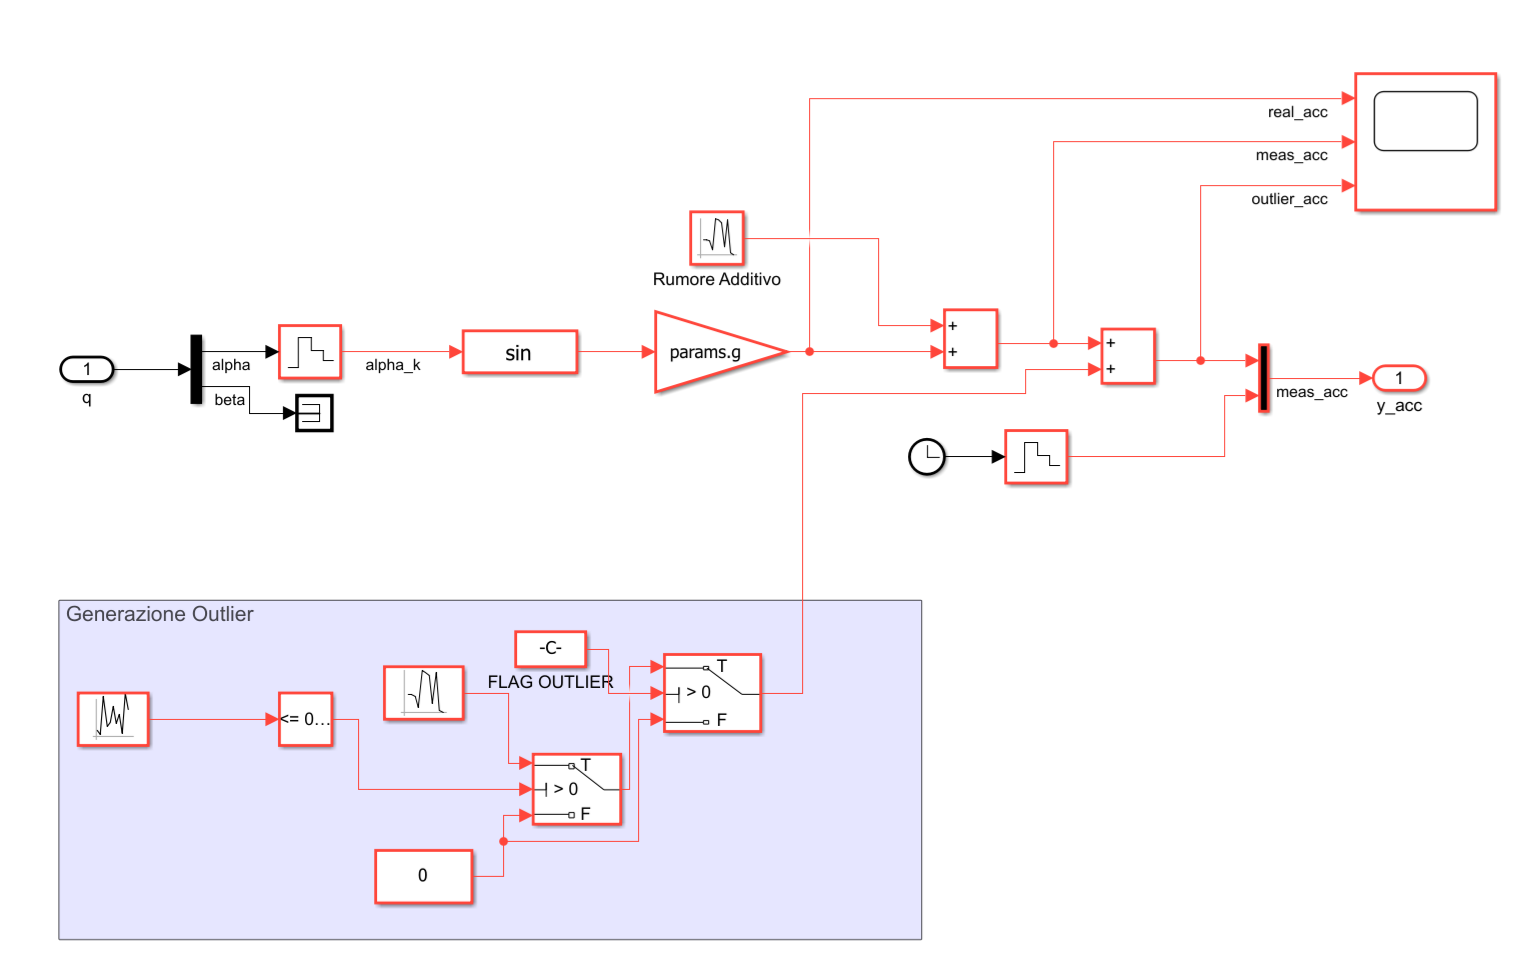
\includegraphics[width=0.8\textwidth]{figures/Schema_acc.png}
    \caption{Schema Simulink accelerometro}
    \label{fig:Schema_simulink_acc}
\end{figure}

\begin{figure}[H]
    \centering
    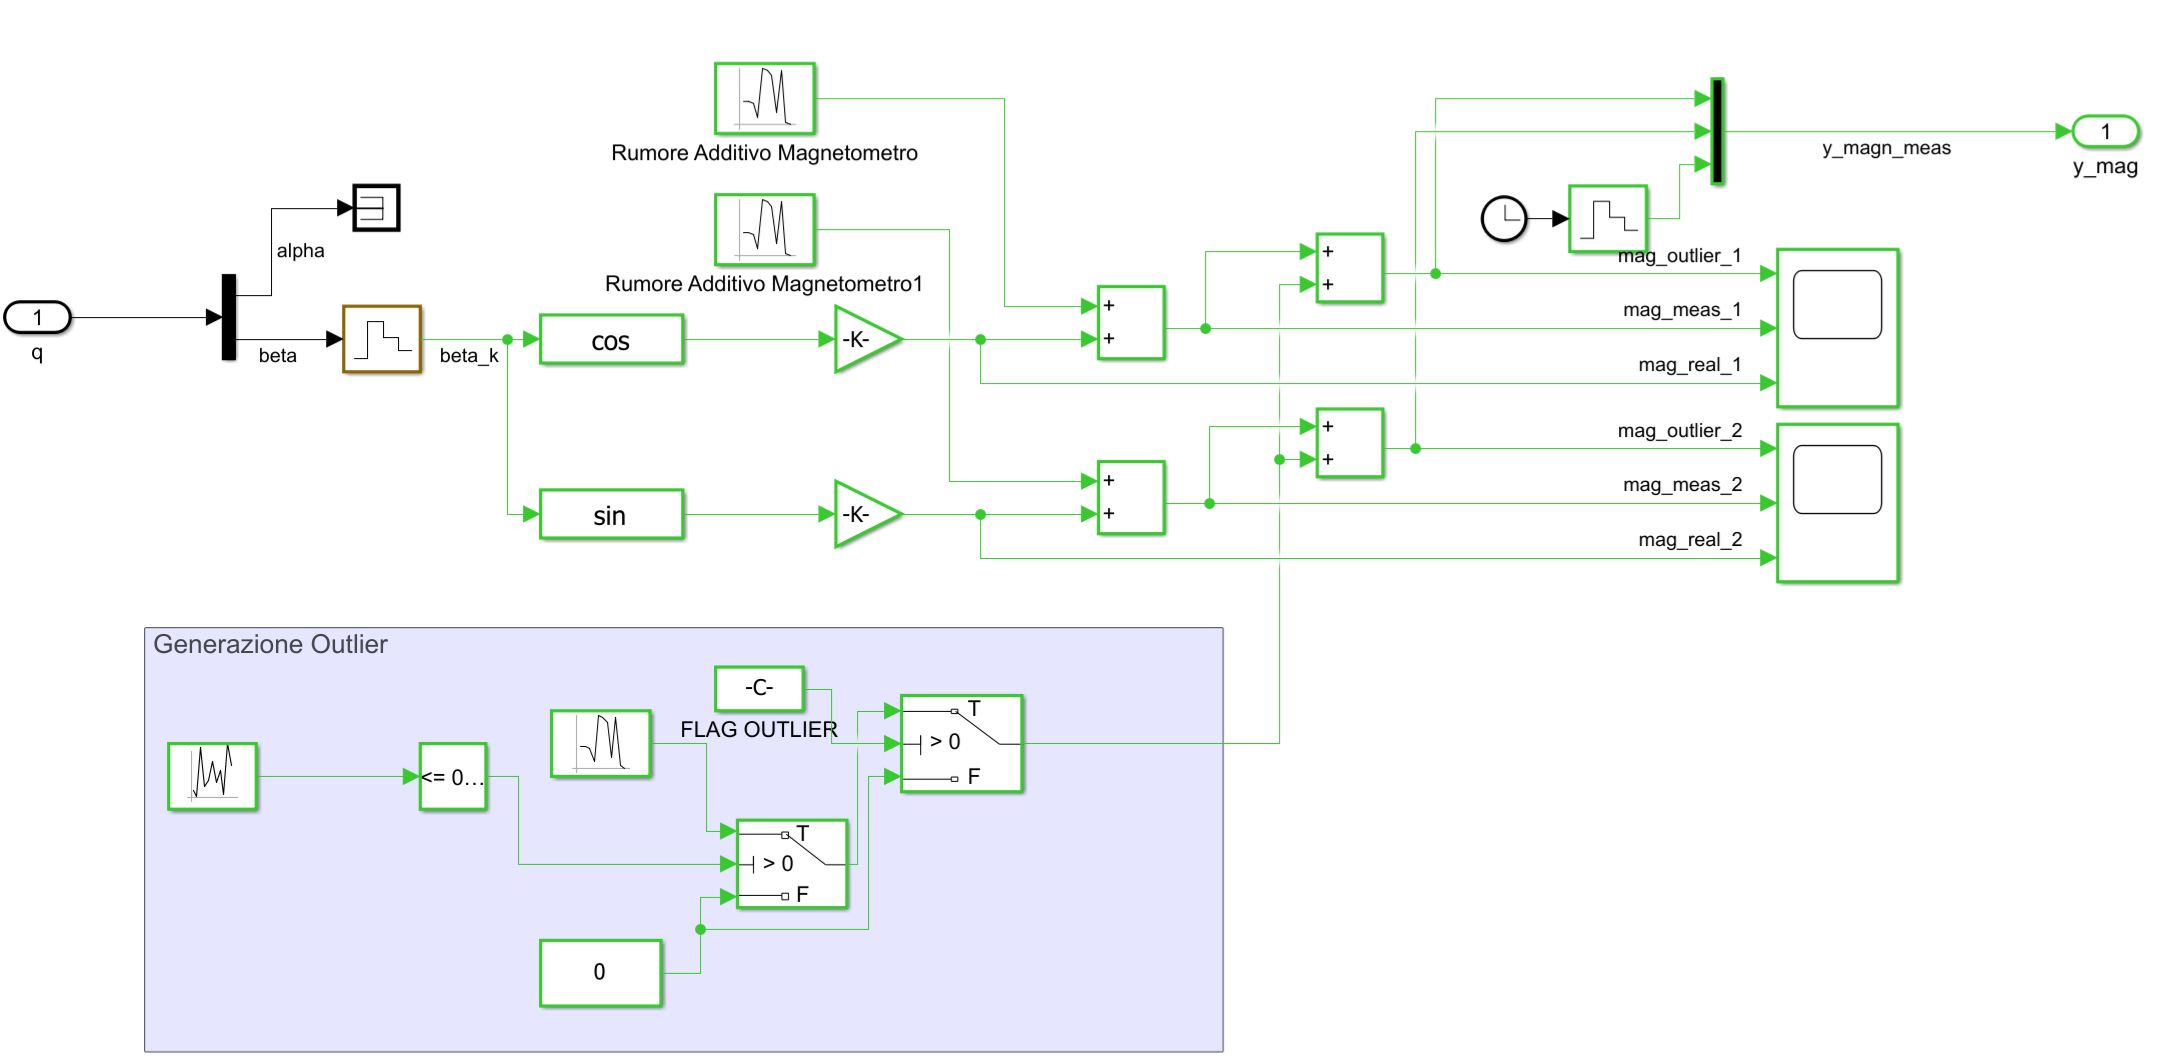
\includegraphics[width=0.8\textwidth]{figures/Schema_magn.png}
    \caption{Schema Simulink magnetometro}
    \label{fig:Schema_simulink_magn}
\end{figure}

\subsubsection{Validazione dei Sensori}

Per validare il modello di osservazione dei sensori è stato eseguito il medesimo test con ingressi nulli illustrato
nella sezione \ref{sec:Validazione_modello}, e sono state monitorate le uscite dei 2 sensori.
In Figura \ref{fig:Acc_input_nullo} è riportato l'andamento delle misure dell'accelerometro
con e senza outlier.

\begin{figure}[H]
    \centering
    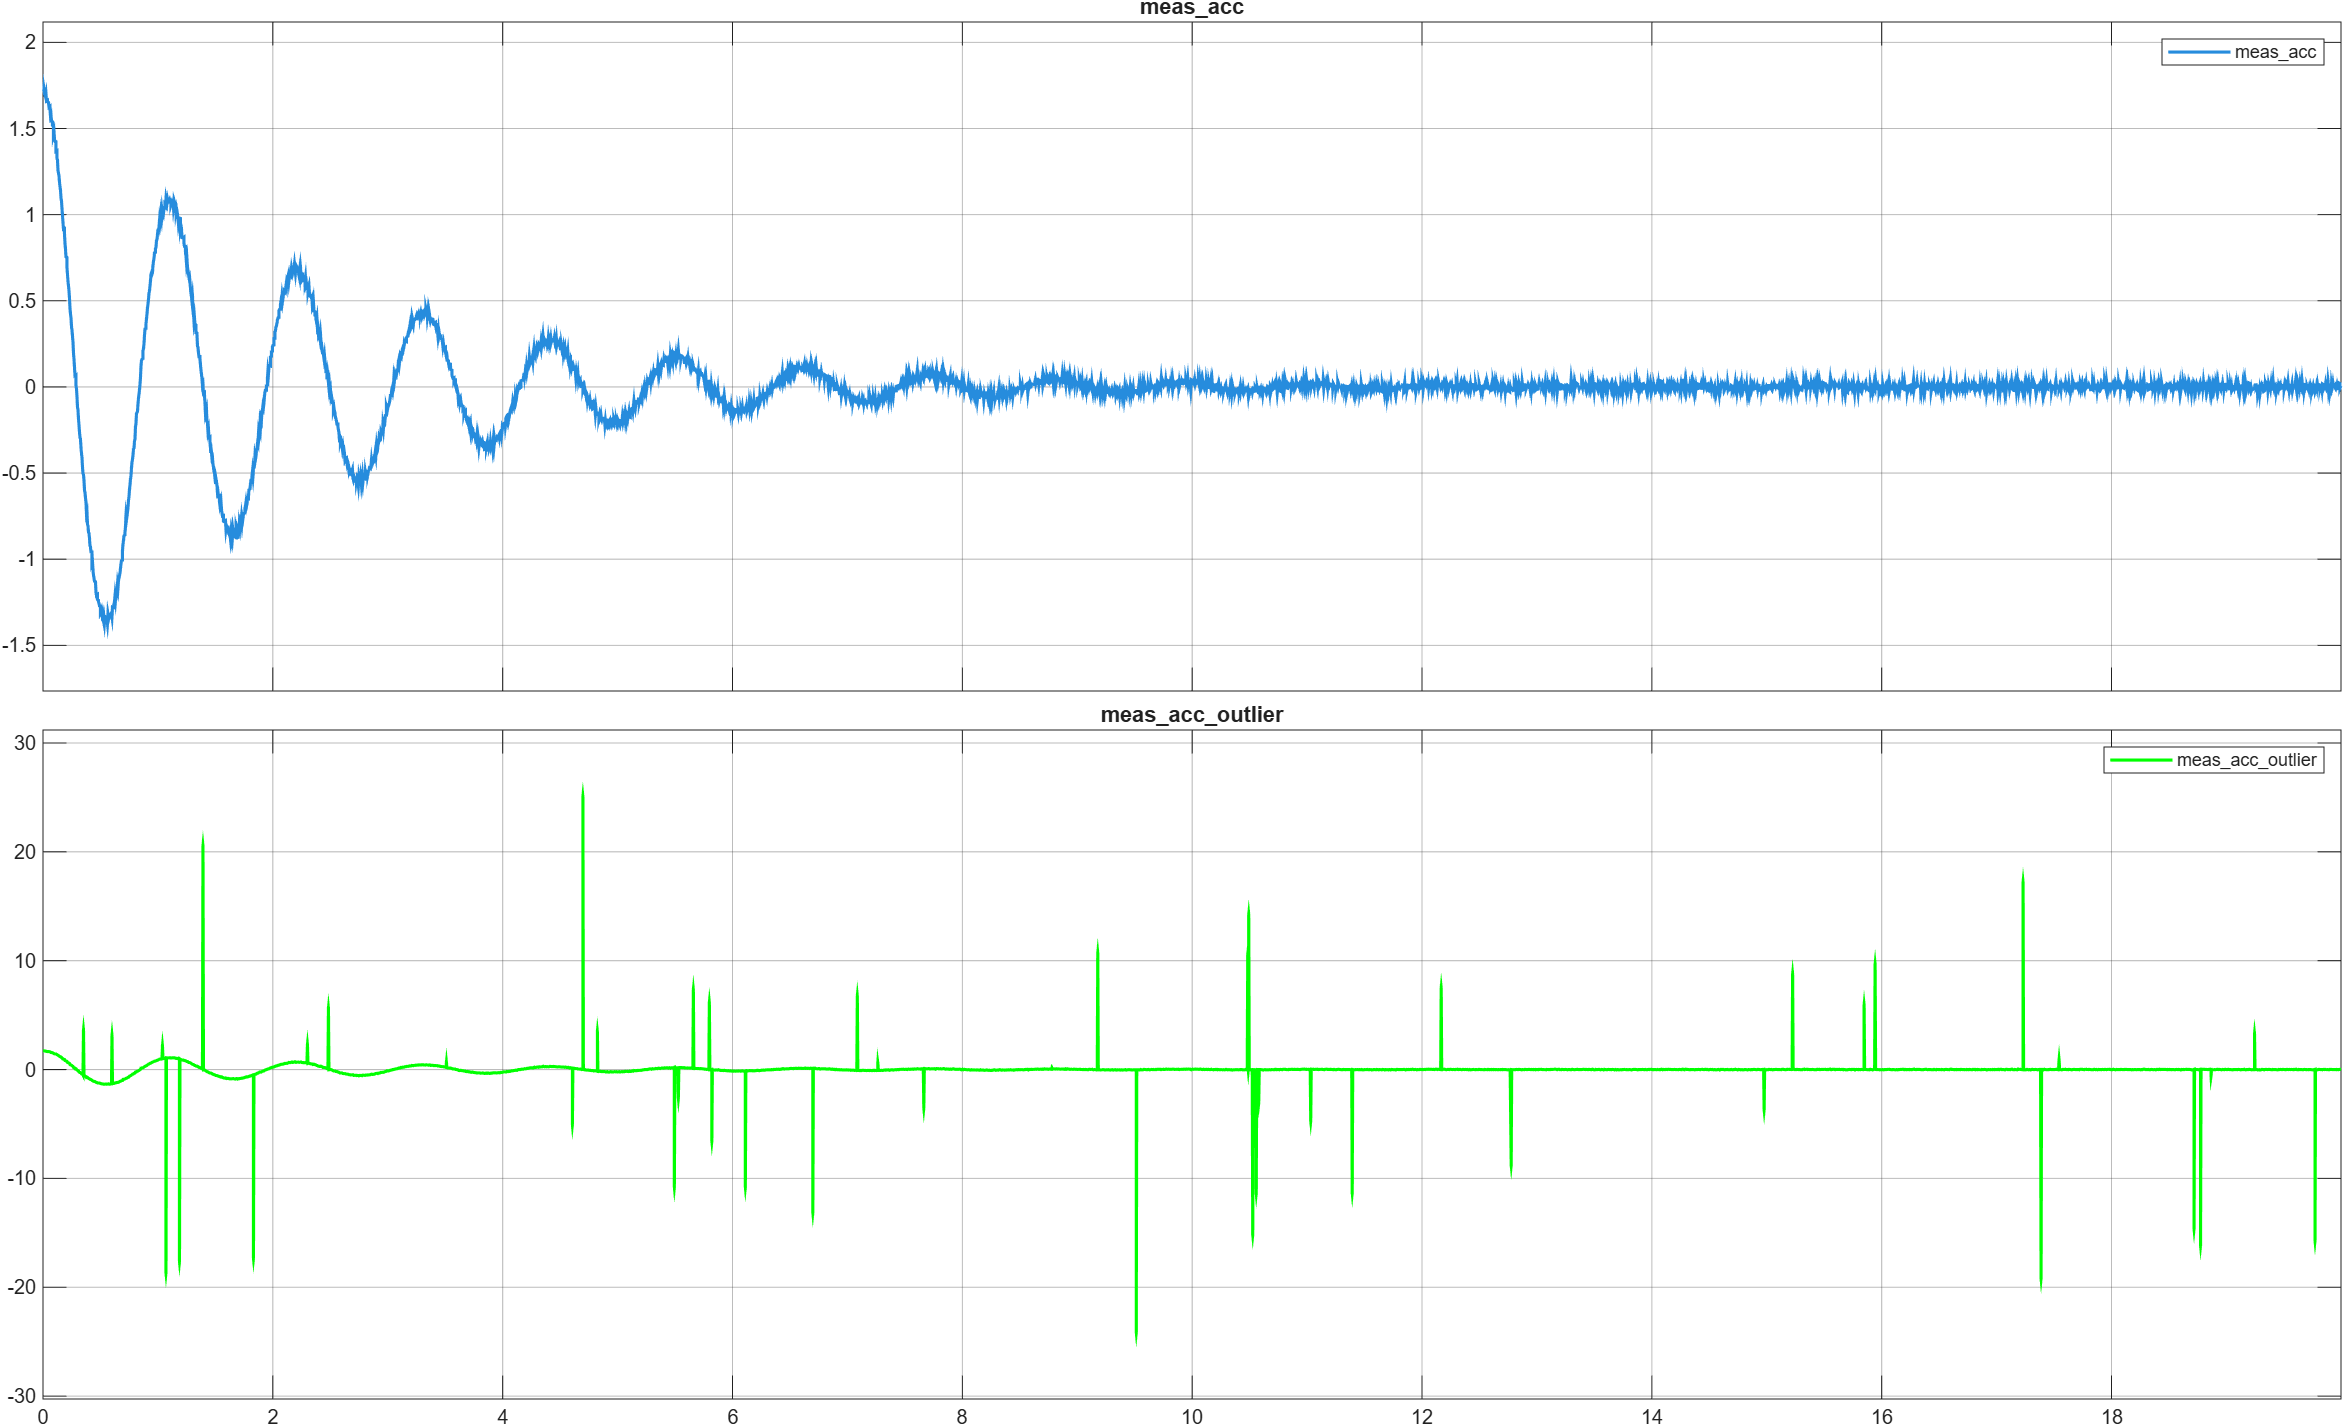
\includegraphics[width=0.9\textwidth]{figures/Acc_input_nullo.png}
    \caption{Misura accelerometro con input nullo}
    \label{fig:Acc_input_nullo}
\end{figure}

Il grafico dell'accelerometro mostra una sinusoide smorzata che converge asintoticamente a zero. L'andamento
è perfettamente coerente con l'equazione di osservazione implementata.

\begin{figure}[H]
    \centering
    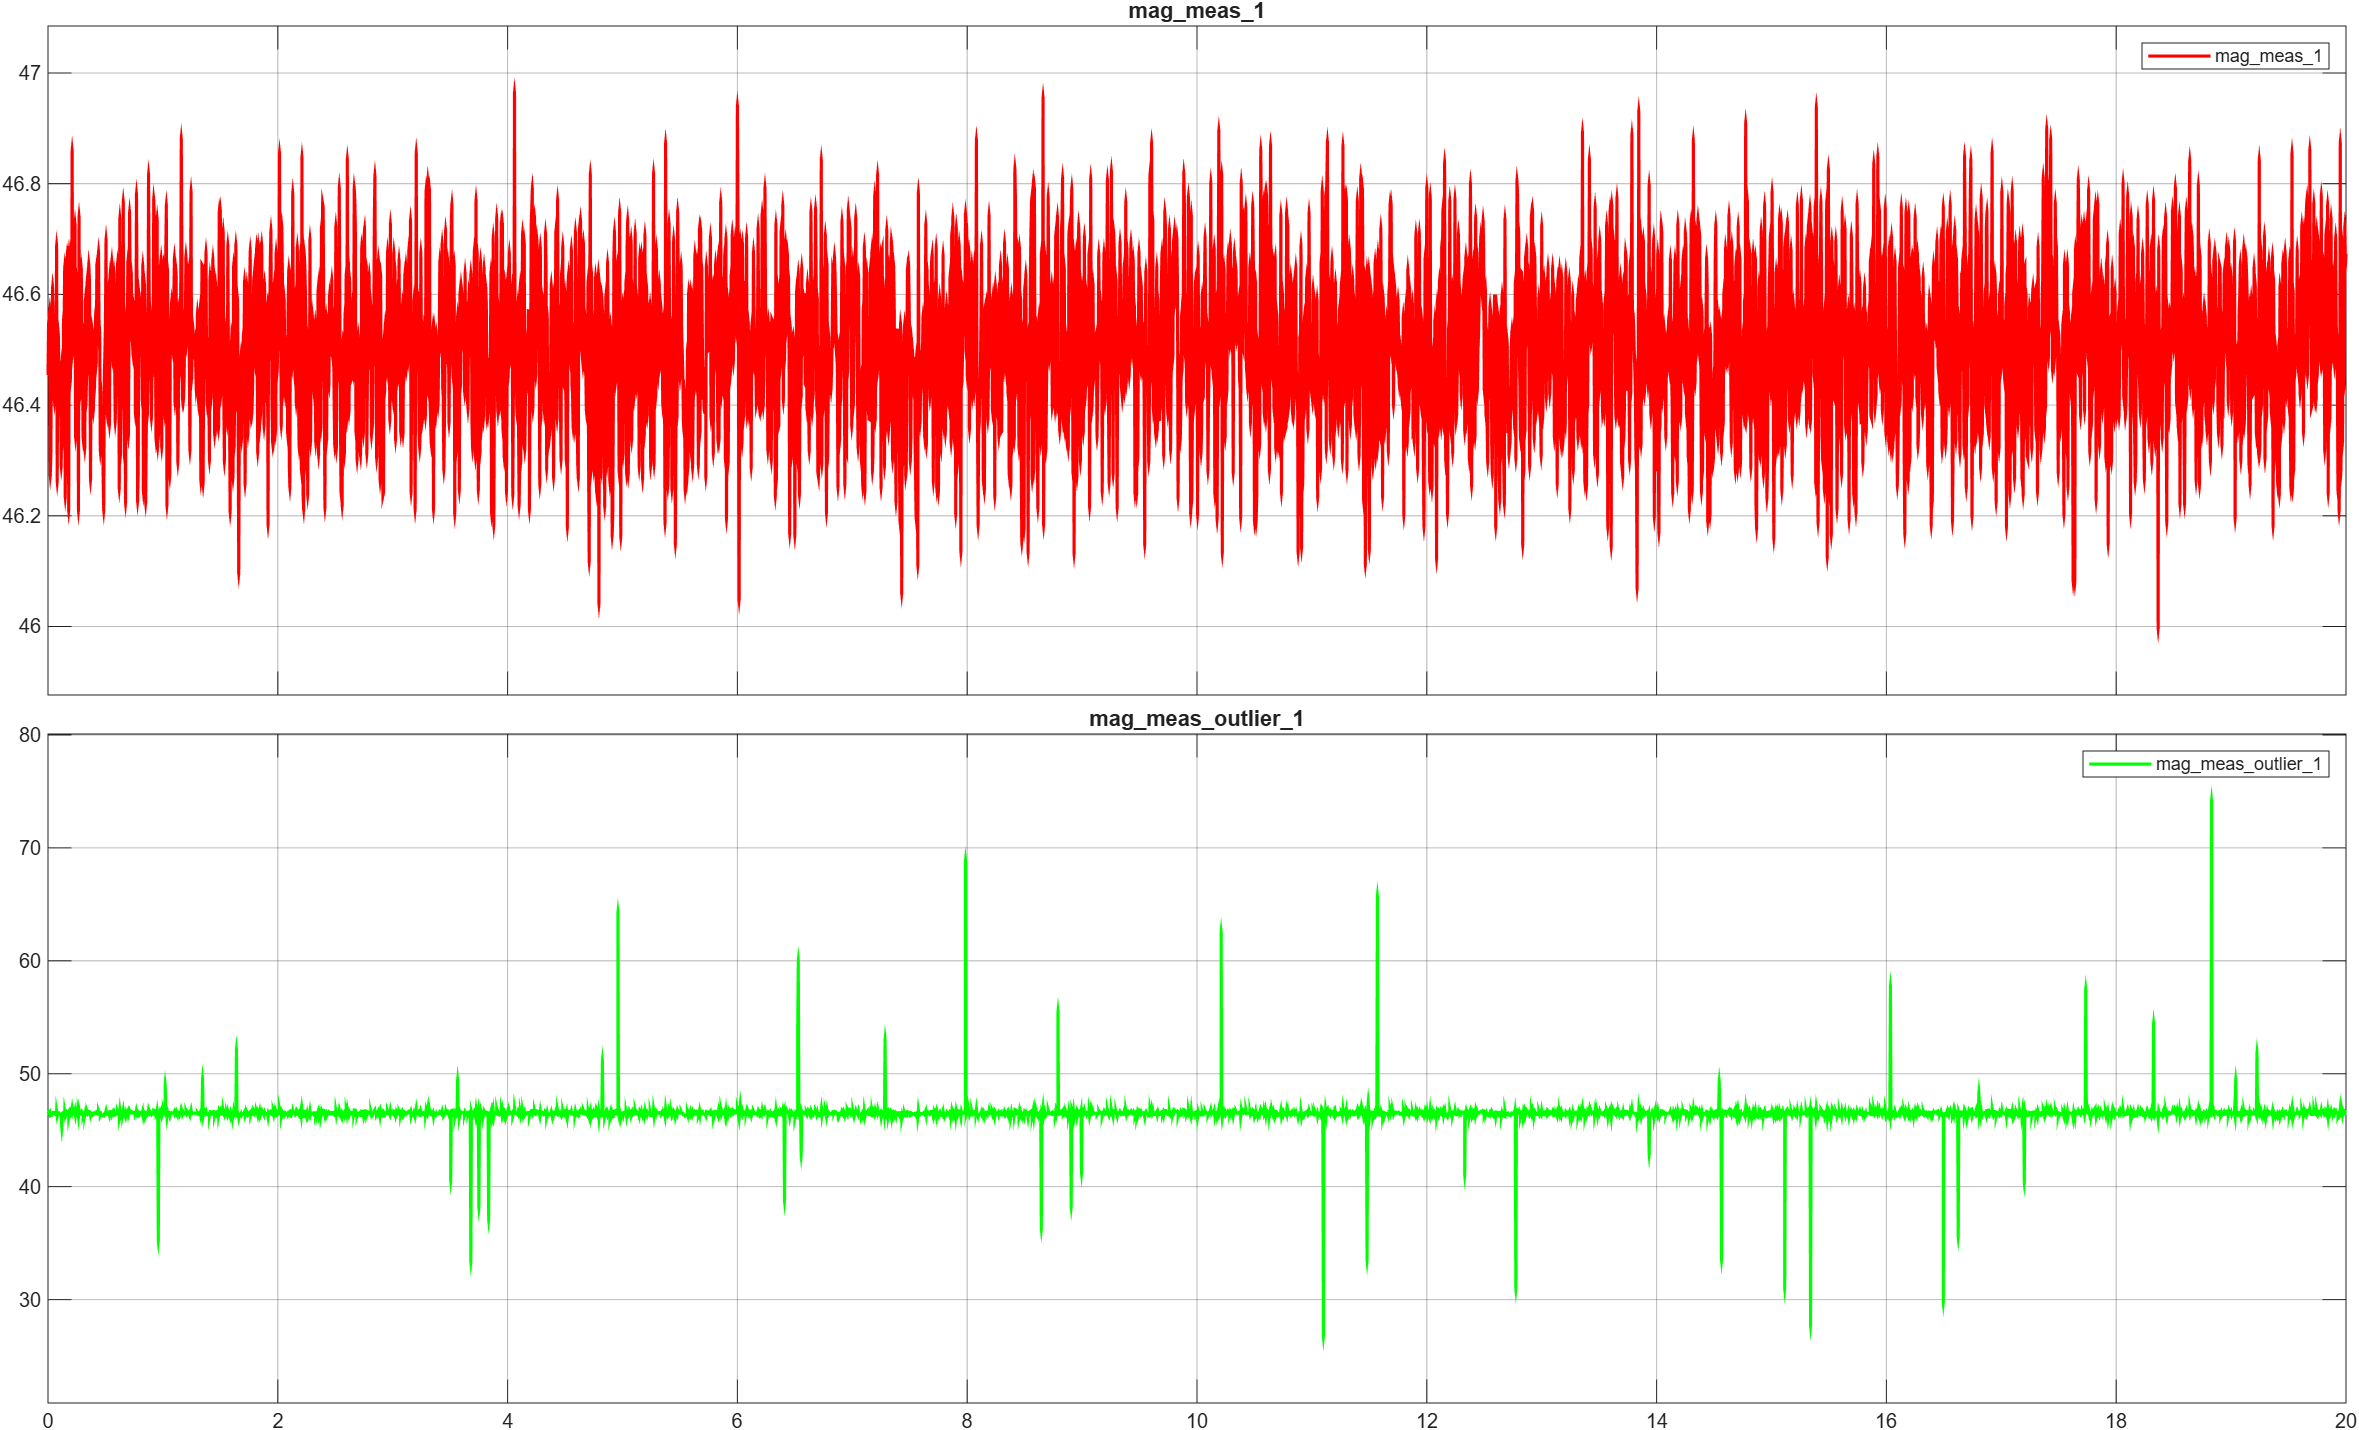
\includegraphics[width=0.9\textwidth]{figures/Mag_input_nullo_1.png}
    \caption{Prima componente della misura di magnetometro con input nullo}
    \label{fig:Mag_input_nullo_1}
\end{figure}


\begin{figure}[H]
    \centering
    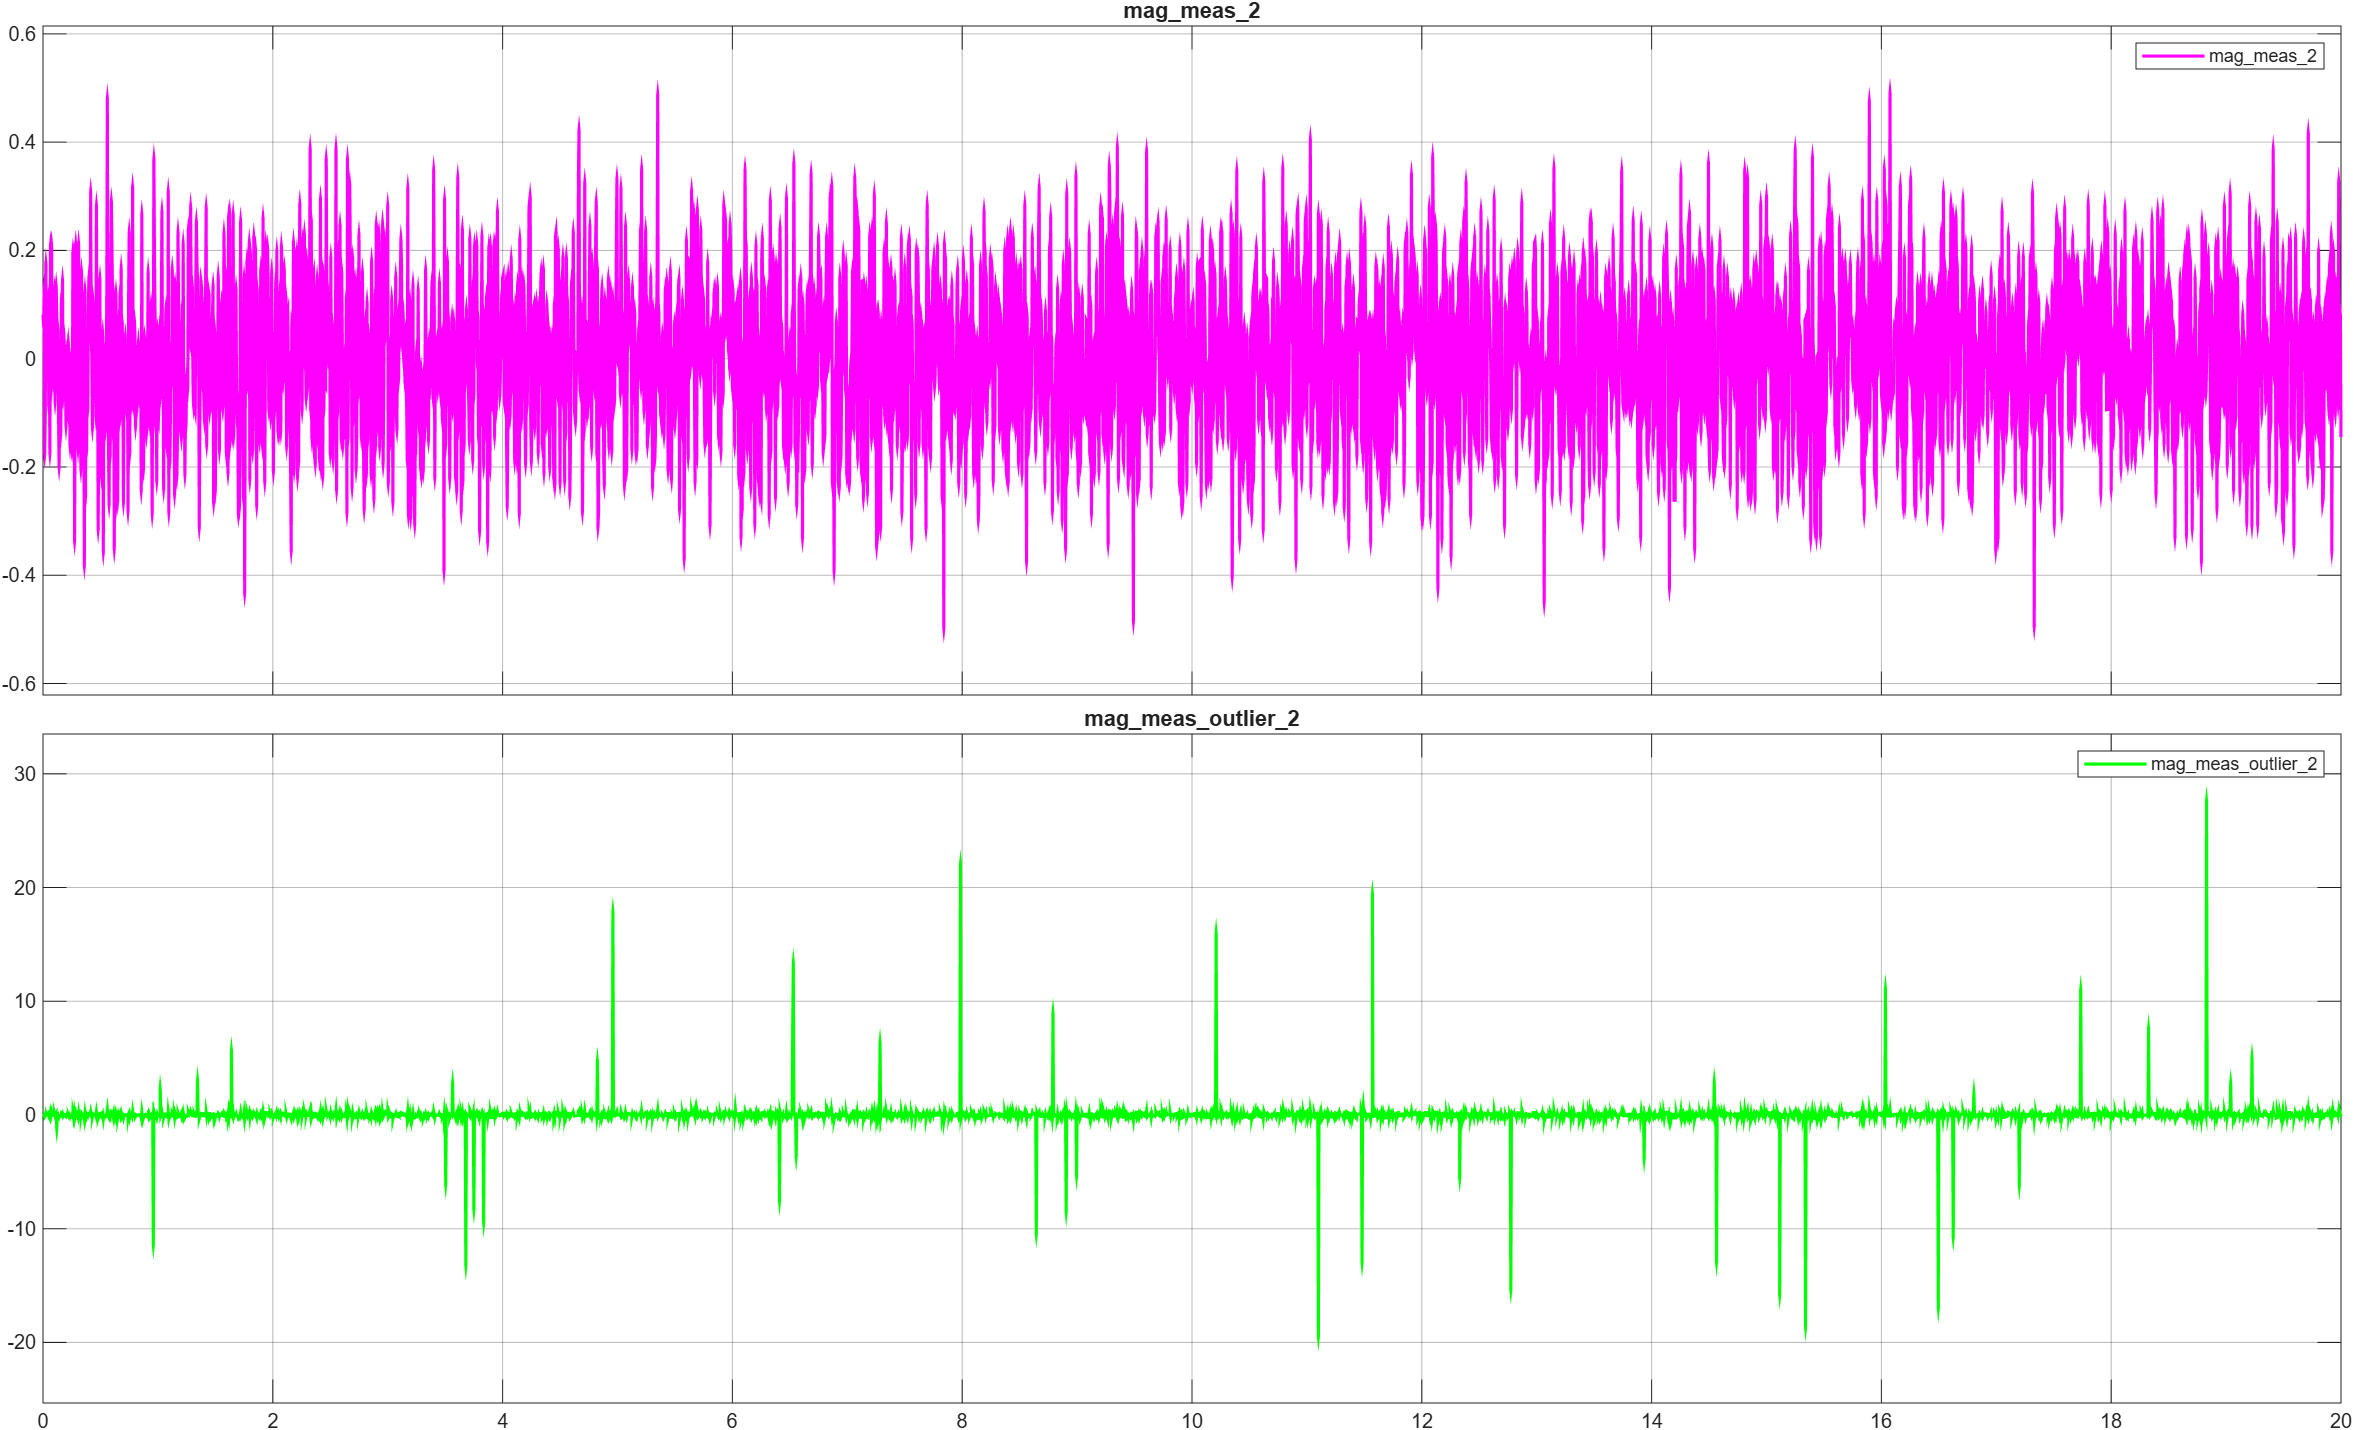
\includegraphics[width=0.9\textwidth]{figures/Mag_input_nullo_2.png}
    \caption{Seconda componente della misura di magnetometro con input nullo}
    \label{fig:Mag_input_nullo_2}
\end{figure}

I grafici relativi al magnetometro mostrano segnali
che validano il modello matematico in assenza di rotazioni sull'asse verticale.
Essendo l'angolo di imbardata costantemente nullo, nelle 2 misure del magnetometro
compaiono soltanto i rumori secondo le specifiche del sensore.


\section{Filtro di Kalman Esteso}
Il filtro di Kalman esteso (EKF) rappresenta una generalizzazione del filtro di Kalman lineare ai sistemi non lineari. L'idea alla base dell'algoritmo consiste nel linearizzare localmente le equazioni del sistema mediante uno sviluppo di Taylor al primo ordine attorno alla stima corrente dello stato.
Nel caso in esame il modello dinamico dell'elicottero presenta non linearità dovute ai termini trigonometrici presenti nelle equazioni del moto e nella funzione di osservazione. Per tale motivo l'utilizzo del filtro di Kalman classico non risulta applicabile direttamente.
L'algoritmo implementato è costituito da due fasi principali:
\begin{enumerate}
\item Predizione dello stato e della covarianza tramite il modello dinamico.
\item Correzione mediante le misure provenienti dai sensori.
\end{enumerate}
Poiché accelerometro e magnetometro operano a frequenze differenti, l'EKF è stato implementato secondo una logica multi-rate. La fase di predizione viene eseguita con il tempo di campionamento del sensore più veloce, mentre la fase di aggiornamento utilizza solamente le misure effettivamente disponibili all'istante corrente.
Di conseguenza la dimensione del vettore delle osservazioni e delle matrici associate alla correzione varia nel tempo. La dimensione della matrice di covarianza dello stato rimane invece costante ed è pari a ($4\times4$), essendo determinata esclusivamente dalla dimensione del vettore di stato.

\subsection{Predizione}
La fase di predizione utilizza il modello dinamico non lineare discretizzato mediante integrazione di Eulero.
La stima dello stato all'istante successivo viene ottenuta mediante la relazione

\begin{equation}
\hat{x}_{k+1|k} = \hat{x}_{k|k} + T_s f(\hat{x}_{k|k},u_k)
\end{equation}

dove $T_s$ rappresenta il tempo di campionamento fondamentale del sistema.
Per descrivere l'incertezza associata agli attuatori viene introdotto un rumore di processo additivo agente sugli ingressi

\begin{equation}
u_k = \bar{u}_k + w_k
\end{equation}

con

\begin{equation}
w_k \sim \mathcal{N}(0,Q).
\end{equation}

La propagazione della covarianza richiede la linearizzazione locale del modello mediante il calcolo della matrice Jacobiana

\begin{equation}
F_k = \frac{\partial f(x,u)}{\partial x} \Bigg|_{\hat{x}_{k|k}}
\end{equation}

e della matrice di ingresso del rumore

\begin{equation}
D_k = \frac{\partial f(x,u)}{\partial w} \Bigg|_{\hat{x}_{k|k}}.
\end{equation}

La covarianza predetta viene quindi aggiornata secondo

\begin{equation}
P_{k+1|k} = F_k P_{k|k} F_k^T + D_k Q D_k^T.
\end{equation}


\subsection{Correzione}
La fase di correzione sfrutta le misure provenienti dall'accelerometro e dal magnetometro per aggiornare la stima predetta.
Il modello di osservazione adottato è

\begin{equation}
y_k = h(x_k) + v_k
\end{equation}

dove $v_k$ rappresenta un rumore gaussiano bianco caratterizzato da covarianza $R$.
L'innovazione viene definita come

\begin{equation}
e_k = y_k - h(\hat{x}_{k|k-1})
\end{equation}

e rappresenta la discrepanza tra misura reale e misura prevista dal modello.
Linearizzando la funzione di osservazione si ottiene la matrice Jacobiana

\begin{equation}
H_k = \frac{\partial h(x)}{\partial x} \Bigg|_{\hat{x}_{k|k-1}}.
\end{equation}

La covarianza dell'innovazione risulta

\begin{equation}
S_k = H_k P_{k|k-1} H_k^T + R_k
\end{equation}

mentre il guadagno di Kalman è dato da

\begin{equation}
K_k = P_{k|k-1} H_k^T S_k^{-1}.
\end{equation}

La stima corretta dello stato viene infine ottenuta tramite

\begin{equation}
\hat{x}_{k|k} = \hat{x}_{k|k-1} + K_k e_k.
\end{equation}

Per garantire una migliore stabilità numerica la matrice di covarianza aggiornata è stata calcolata utilizzando la forma di Joseph,
che preserva la simmetria e la definita positività della matrice $P$.

\subsubsection{Reiezione delle misure spurie mediante distanza di Mahalanobis}
Durante il funzionamento reale di un sistema di stima possono verificarsi misure anomale dovute a disturbi elettromagnetici, errori di acquisizione o malfunzionamenti temporanei dei sensori. L'utilizzo diretto di tali misure nella fase di correzione può causare errori significativi nella stima dello stato o addirittura portare alla divergenza del filtro.
Per limitare tale fenomeno è stata implementata una logica di validazione statistica basata sulla distanza di Mahalanobis. Tale grandezza misura quanto una determinata innovazione risulti compatibile con la distribuzione statistica prevista dal filtro.
Nel caso generale la distanza di Mahalanobis è definita come
\begin{equation}
D_M=
\sqrt{
e_k^TS_k^{-1}e_k
}
\end{equation}
dove ($e_k$) rappresenta il vettore di innovazione e ($S_k$) la relativa matrice di covarianza.
Nel progetto sviluppato si è scelto di effettuare un controllo separato per accelerometro e magnetometro. Tale approccio permette di rigettare selettivamente il sensore affetto da un'anomalia senza compromettere l'utilizzo delle informazioni provenienti dagli altri dispositivi.
Qualora la distanza di Mahalanobis superi il valore di soglia, la misura viene considerata non affidabile e viene esclusa dall'aggiornamento del filtro. In tal modo si ottiene un significativo incremento della robustezza dell'algoritmo in presenza di misure spurie.


\section{Filtro di Kalman Unscented}
Sebbene l'EKF rappresenti uno degli strumenti più diffusi per la stima di sistemi non lineari, le sue prestazioni dipendono fortemente dalla qualità della linearizzazione locale. In presenza di dinamiche fortemente non lineari la propagazione degli errori ottenuta mediante lo sviluppo di Taylor può risultare inaccurata.
Per superare tale limitazione è stato implementato un filtro di Kalman Unscented (UKF). Questo approccio evita completamente il calcolo delle matrici Jacobiane e utilizza invece la Trasformata Unscented per propagare media e covarianza attraverso il modello non lineare.
L'idea fondamentale consiste nel rappresentare la distribuzione di probabilità dello stato mediante un insieme deterministico di punti, detti Sigma Points, opportunamente scelti affinché abbiano la stessa media e covarianza della distribuzione originale.
Tali punti vengono propagati attraverso il modello non lineare e successivamente ricombinati per ottenere una stima accurata delle statistiche dello stato.
L'approccio Unscented risulta particolarmente adatto al caso dell'elicottero 2DOF, caratterizzato dalla presenza di non linearità trigonometriche e da una matrice di inerzia dipendente dall'assetto.


\subsection{Predizione mediante stato aumentato}
Nel caso in esame il rumore di processo non agisce direttamente sulle variabili di stato, ma sugli ingressi di controllo associati ai due motori.
Per descrivere correttamente tale fenomeno è stata adottata una formulazione a stato aumentato.
Il vettore di stato esteso assume quindi la forma

\begin{equation}
x_a =
\begin{bmatrix}
x \\
w
\end{bmatrix}
=
\begin{bmatrix}
\alpha \\
\dot{\alpha} \\
\beta \\
\dot{\beta} \\
w_{F_1} \\
w_{F_2}
\end{bmatrix}
\end{equation}

dove $w_{F_1}$ e $w_{F_2}$ rappresentano i rumori associati ai due attuatori.
La covarianza aumentata risulta

\begin{equation}
P_a =
\begin{bmatrix}
P & 0 \\
0 & Q
\end{bmatrix}.
\end{equation}

A partire da tale matrice vengono generati $2n+1$ Sigma Points secondo la relazione

\begin{equation}
\chi_0 = \hat{x}
\end{equation}
\begin{equation}
\chi_i = \hat{x} + \sqrt{n+\kappa} \, \Gamma_i
\end{equation}
\begin{equation}
\chi_{i+n} = \hat{x} - \sqrt{n+\kappa} \, \Gamma_i
\end{equation}

dove $\Gamma_i$ rappresenta la $i$-esima colonna della radice quadrata della matrice di covarianza.
Ogni Sigma Point viene successivamente propagato attraverso il modello dinamico non lineare dell'elicottero ottenendo una nuvola di punti che approssima l'evoluzione della distribuzione di probabilità dello stato.
La nuova media e la nuova covarianza vengono infine calcolate come combinazione pesata dei Sigma Points propagati.


\subsection{Correzione Unscented}
La fase di aggiornamento utilizza il medesimo principio della Trasformata Unscented applicato al modello di osservazione.
I Sigma Points ottenuti nella fase di predizione vengono propagati attraverso la funzione di misura

\begin{equation}
y = h(x)
\end{equation}

ottenendo una distribuzione delle osservazioni previste.
Nel caso dell'elicottero tale funzione è costituita dal modello accelerometrico

\begin{equation}
y_{acc} = g\sin(\alpha)
\end{equation}

e dal modello magnetometrico

\begin{equation}
y_{magn} =
\begin{bmatrix}
M_0\cos(\beta) \\
-M_0\sin(\beta)
\end{bmatrix}.
\end{equation}

Dalla propagazione dei Sigma Points si ottengono la media prevista delle misure, la covarianza delle osservazioni e la covarianza incrociata stato-misura.
Il guadagno di Kalman Unscented viene quindi calcolato come

\begin{equation}
K = P_{xy} P_{yy}^{-1}
\end{equation}

e utilizzato per aggiornare stato e covarianza secondo

\begin{equation}
\hat{x}^{+} = \hat{x}^{-} + K(y-\hat{y})
\end{equation}
\begin{equation}
P^{+} = P^{-} - K P_{yy} K^T.
\end{equation}

L'assenza di linearizzazioni consente all'UKF di mantenere una maggiore accuratezza
nella propagazione delle statistiche anche in presenza di dinamiche fortemente non lineari.

\section{Rauch-Tung-Striebel Smoother}
Lo smoother Rauch-Tung-Striebel (RTS) rappresenta un'estensione del filtro di Kalman che consente di migliorare la stima degli stati passati sfruttando informazioni disponibili in istanti successivi.
A differenza di EKF e UKF, che operano in tempo reale utilizzando esclusivamente misure presenti e passate, il filtro RTS è un algoritmo offline che richiede la disponibilità dell'intera sequenza temporale delle osservazioni.
L'algoritmo è composto da due fasi:
\begin{enumerate}
\item filtraggio in avanti;
\item regolarizzazione all'indietro.
\end{enumerate}
Nella prima fase viene eseguito il filtro di Kalman producendo, per ogni istante temporale, le stime corrette $\hat{x}_{k|k}$ e le relative covarianze $P_{k|k}$.
Successivamente viene effettuata una scansione inversa della traiettoria a partire dall'ultimo campione disponibile.
Definendo

\begin{equation}
C_k = P_{k|k} F_{k+1}^{T} P_{k+1|k}^{-1}
\end{equation}

si ottiene il guadagno di smoothing utilizzato per correggere le stime passate.
La stima regolarizzata assume quindi la forma

\begin{equation}
\hat{x}_{k|N} = \hat{x}_{k|k} + C_k \left( \hat{x}_{k+1|N} - \hat{x}_{k+1|k} \right)
\end{equation}

mentre la covarianza associata viene aggiornata secondo

\begin{equation}
P_{k|N} = P_{k|k} + C_k \left( P_{k+1|N} - P_{k+1|k} \right) C_k^T.
\end{equation}

Grazie all'utilizzo delle informazioni future, lo smoother RTS è in grado di ridurre
il rumore residuo presente nelle stime e migliorare
la ricostruzione delle variabili non direttamente osservabili.

\section{Analisi dei risultati}
Per valutare le prestazioni degli algoritmi sviluppati sono stati analizzati gli andamenti temporali degli stati stimati, delle matrici di covarianza e delle innovazioni.
Le simulazioni sono state effettuate utilizzando traiettorie ottenute mediante ingressi sinusoidali applicati ai due motori, in modo da eccitare simultaneamente le dinamiche di pitch e yaw.
L'errore di stima è stato definito come

\begin{equation}
e_x(t) = x_{vero}(t) - \hat{x}(t)
\end{equation}

e valutato separatamente per ciascuna componente dello stato.
Particolare attenzione è stata dedicata all'analisi delle variabili angolari. 
Poiché gli angoli sono definiti modulo $2\pi$, gli errori associati alle componenti 
$\alpha$ e $\beta$ sono stati normalizzati all'interno dell'intervallo $[-\pi,\pi]$ 
al fine di evitare discontinuità artificiali dovute al fenomeno del wrapping.
Oltre all'errore di stima sono state analizzate le innovazioni prodotte dai filtri, 
verificandone la consistenza statistica mediante test di bianchezza basati sull'autocorrelazione
campionaria.
L'obiettivo di tale analisi consiste nel verificare che le informazioni contenute
nelle misure siano state correttamente sfruttate dal filtro e che non permangano dinamiche
sistematiche non modellate.


\subsection{Prestazioni dell'EKF}
Le simulazioni effettuate mostrano che il filtro di Kalman esteso è in grado di ricostruire correttamente l'evoluzione delle variabili di stato dell'elicottero.
Le stime ottenute risultano generalmente sovrapposte alle traiettorie reali e gli errori rimangono confinati entro intervalli compatibili con l'incertezza introdotta dai rumori di processo e misura.
Le componenti associate al pitch presentano le migliori prestazioni, grazie alla presenza di una misura accelerometrica direttamente correlata all'angolo ($\alpha$).
La stima dello yaw risulta invece più complessa, poiché dipende esclusivamente dalle informazioni fornite dal magnetometro. Tale sensore introduce una maggiore sensibilità agli errori di modellazione e ai disturbi esterni, rendendo la componente ($\beta$) maggiormente critica rispetto alle altre variabili.
L'introduzione della logica di reiezione basata sulla distanza di Mahalanobis ha consentito di eliminare efficacemente le misure spurie senza compromettere la stabilità complessiva del filtro.

\subsection{Prestazioni dell'UKF}
Il filtro di Kalman Unscented ha mostrato prestazioni complessivamente comparabili o superiori rispetto all'EKF.
L'assenza di linearizzazioni locali consente infatti di propagare in maniera più accurata le statistiche dello stato attraverso il modello dinamico non lineare.
Tale vantaggio risulta particolarmente evidente durante le manovre caratterizzate da variazioni simultanee di pitch e yaw, nelle quali gli effetti di accoppiamento tra le dinamiche diventano più pronunciati.
L'UKF presenta inoltre una maggiore robustezza nei confronti delle approssimazioni numeriche associate alle matrici Jacobiane, completamente assenti nell'implementazione Unscented.
Dal punto di vista computazionale, tuttavia, il costo richiesto dall'UKF risulta superiore rispetto a quello dell'EKF, poiché ad ogni iterazione è necessario generare e propagare un insieme completo di Sigma Points.
Nonostante tale incremento di complessità, le prestazioni ottenute giustificano l'utilizzo dell'approccio Unscented in applicazioni caratterizzate da elevate non linearità.

\subsection{Confronto tra EKF e UKF}
Il confronto tra i due algoritmi evidenzia differenze principalmente riconducibili al metodo utilizzato per la propagazione dell'incertezza.
L'EKF utilizza una linearizzazione locale ottenuta tramite sviluppo di Taylor al primo ordine. Tale approssimazione risulta generalmente adeguata quando il sistema opera in prossimità di condizioni quasi lineari.
L'UKF, al contrario, evita completamente il processo di linearizzazione e sfrutta la Trasformata Unscented per propagare direttamente media e covarianza attraverso le equazioni non lineari.
Dal punto di vista dell'accuratezza, l'UKF fornisce generalmente stime leggermente migliori delle variabili maggiormente influenzate dalle non linearità del modello. Tale vantaggio risulta particolarmente evidente nelle condizioni operative caratterizzate da ampie escursioni degli angoli o da forti accoppiamenti dinamici.
L'EKF presenta invece una minore complessità computazionale e una struttura più semplice da implementare e validare.
Nel contesto del presente progetto entrambi i filtri hanno mostrato prestazioni soddisfacenti, consentendo una corretta ricostruzione dello stato dell'elicottero.


\subsection{Confronto tra EKF e RTS}
L'analisi comparativa tra EKF e RTS evidenzia come le stime prodotte dai due algoritmi risultino generalmente molto simili.
Lo smoother RTS introduce un miglioramento principalmente nelle componenti caratterizzate da maggiore rumore e nelle derivate angolari, che risultano più regolari rispetto alle corrispondenti stime filtrate.
Tale comportamento è una diretta conseguenza dell'utilizzo delle informazioni future durante la fase di smoothing.
I vantaggi dell'RTS diventano particolarmente evidenti nelle applicazioni offline, quali analisi sperimentali, identificazione parametrica e post-processing di dati acquisiti.
Viceversa, nelle applicazioni in tempo reale il filtro non può essere utilizzato poiché richiede la disponibilità dell'intera sequenza di osservazioni.
I risultati ottenuti mostrano che l'EKF fornisce già una stima sufficientemente accurata per applicazioni online, mentre l'RTS consente di ottenere una ricostruzione più regolare e statisticamente consistente delle traiettorie.


\section{Conclusioni}
Nel presente lavoro sono stati sviluppati e validati differenti algoritmi di stima applicati ad un modello non lineare di elicottero a due gradi di libertà.
Partendo dalla realizzazione del modello dinamico e della relativa sensoristica virtuale, sono stati implementati un filtro di Kalman esteso, un filtro di Kalman Unscented ed uno smoother di Rauch-Tung-Striebel.
L'analisi dei risultati ha mostrato come tutti gli algoritmi siano in grado di ricostruire correttamente lo stato del sistema anche in presenza di rumori di processo, rumori di misura e misure spurie.
L'EKF si è dimostrato una soluzione efficace e relativamente semplice da implementare, mentre l'UKF ha evidenziato una maggiore accuratezza nella gestione delle non linearità del modello. Lo smoother RTS ha infine consentito di migliorare ulteriormente la qualità delle stime attraverso un'elaborazione offline delle traiettorie.
Particolare attenzione è stata dedicata alla robustezza numerica dell'implementazione, introducendo tecniche di validazione statistica mediante distanza di Mahalanobis, gestione multi-rate delle misure e procedure di stabilizzazione numerica basate sulla decomposizione ai valori singolari.
I risultati ottenuti confermano la validità delle metodologie adottate e mostrano come gli strumenti di sensor fusion basati sul filtro di Kalman rappresentino una soluzione efficace per la stima dello stato di sistemi aeronautici caratterizzati da dinamiche non lineari.

\end{document}
